\documentclass[a4paper,12pt,oneside]{report}
\usepackage{OvidiusFMI}
\usepackage{times}
\usepackage{graphicx}
\usepackage{hyperref}
\usepackage{color,xcolor}
\usepackage{amsmath}
\usepackage{framed}
\usepackage{indentfirst}
\usepackage{enumerate}
\usepackage[shortlabels]{enumitem}
\usepackage{listings}
\usepackage{amsmath,amsfonts,amssymb,amsthm,epsfig,epstopdf,url,array}
\usepackage{multicol,multirow}
\definecolor{code}{rgb}{0.97,0.97,0.97}
\lstdefinestyle{customc}{
  belowcaptionskip=1\baselineskip,
  backgroundcolor=\color{code},
  breaklines=true,
%  frame=L,
%  xleftmargin=\parindent,
  language=C,
  showstringspaces=false,
  morekeywords={bool,
  				 glutMainLoop, glutIdleFunc, glMatrixMode, glLoadIdentity, glPushMatrix, glPopMatrix, 
  				 glBegin, glEnd, glTranslatef, glRotatef, glScalef, glColor3f, glColor4f, glutSolidCube, glutWireCube, glutSolidSphere,
  				 glutWireSphere, glutSolidCone,glutSetWindowTitle,glutGet,glClear,glutSwapBuffers,glDepthFunc,
  				 glutWireCone, glutSolidTorus, glutWireTorus, glutSolidDodecahedron, glutWireDodecahedron,
  				 glutSolidOctahedron, glutWireOctahedron, glutSolidTetrahedron, glutWireTetrahedron, 
  				 glVertex3f,glVertex2f,glPointSize,
  				 glutSolidIcosahedron, glutWireIcosahedron, glutSolidTeapot, glutWireTeapot,glutReshapeFunc,
  				 glFlush, gluPerspective, glutPostRedisplay, glutInit, glutKeyboardFunc,glutKeyboardUpFunc,
  				 glutInitWindowSize, glutInitWindowPosition, glutInitDisplayMode, glutCreateWindow, glutDisplayFunc,glutPassiveMotionFunc,
  				 glClear,glTexCoord2f,
  				 glEnable, glDisable, glLightfv, glMaterialfv, glCullFace,glViewport,
  				 glFrontFace,glColor3ub, glShadeModel,
  				 glGenLists, glGetFloatv,glGentextures,glTexImage2D,glTexParameteri, free, glDeleteTextures,
  				 glLineStipple, glLineWidth, glBindTexture,glGenTextures,
  				 glNewList, glEndList, glCallList,
  				 glMap1f,glEvalCoord1f,glMapGrid1d,glEvalMesh1,glMap2f,glEvalCoord2f,glMapGrid2f,glEvalMesh2,
  				 gluBeginTrim, gluEndTrim, gluPwlCurve,glHint,
  				 GLUnurbsObj, gluBeginSurface, gluNurbsSurface, gluEndSurface, gluNewNurbsRenderer, 									gluNurbsProperty,gluQuadricNormals,
  				 glNormal3f,
  				 gluQuadricTexture,GLUquadricObj,gluSphere,
  				 glPolygonMode, glBlendFunc,glFogi,glFogiv,glFogfv,
  				 GLfloat, GLdouble, GLint,GLuint, GLushort,GLubyte, glRasterPos2f,
  				 gluBeginCurve, gluNurbsCurve, gluEndCurve,
  				 glOrtho, gluLookAt, glutBitmapCharacter, 
  				 glInitNames, glPushName, glLoadName, glSelectBuffer, glRenderMode,gluPickMatrix, glGetIntegerv, glutMouseFunc,glutMotionFunc,system,
  				 glPushAttrib, glPopAttrib, glMultMatrixf, sprintf, glClearStencil, glStencilFunc,glStencilOp,glStencilMask,glColorMask,glActiveStencilFaceEXT,fprintf},  
%   numbers=left,                    % where to put the line-numbers; possible values are (none, left, right)
  %numbersep=5pt,                   % how far the line-numbers are from the code
  %numberstyle=\tiny\color{code}, % the style that is used for the line-numbers
  basicstyle=\footnotesize\ttfamily,
  keywordstyle=\bfseries\color{green!40!black},
  commentstyle=\itshape\color{purple!40!black},
  identifierstyle=\color{blue},
  stringstyle=\color{orange},
}

\lstset{escapechar=@,style=customc}


\newtheorem{definition}{Defini\c tie}
\newtheorem{problem}{Problema}
\newtheorem{proposition}{Propozi\c tie}
\newtheorem{demonstration}{Demonstra\c tie}
\newtheorem{example}{Exemplu}
\newtheorem{theorem}{Teorem\u a}
\newtheorem{remark}{Observa\c{t}ie}
\newtheorem{lemma}{Lem\u{a}}
\newtheorem{solve}{Rezolvare}
\newtheorem{corollary}{Corolar}
\renewcommand*{\proofname}{\rm\bf{Demonstra\c{t}ie}:}

\facultatea{Matematic\u a \c si Informatic\u a}
\specializarea{Informatic\u a}
\teza{Diserta\c{t}ie}
\titlu{Diserta\c{t}ie}
\coordonatorPrincipal{Prof. univ. Cosma Lumini\c ta}
\autor{T\u anase Ramona Elena}
\data{2021}

\begin{document}
\maketitle

\pagenumbering{roman}
\tableofcontents

\pagenumbering{arabic}
%
%
%CAPITOLUL 1
%
%
\chapter{No\c{t}iuni teoretice}

\section{Defini\c{t}ii. Propriet\u{a}\c{t}i}

Studiul funcțiilor convexe de o variabil\u {a} reala\u {a}, ofer\u{a} o imagine excelent\u {a} a frumuse\c {t}ii \c{s}i fascina\c{t}iei matematicii avansate. Vom g\u{a}si aici o mare varietate de rezultate bazate pe argumente simple \c{s}i intuitive care au aplica\c{t}ii remarcabile.

\^{I}n continuare vom nota cu I un interval nedegenerat din \(\mathbb{R}\).

\begin{definition}

O functie \(f: I \rightarrow \mathbb{R}\) se nume\c{s}te convex\u{a} dac\u{a},
\begin{displaymath}
f \left ( \left ( 1 - \lambda  \right )x + \lambda y \right )\leq \left ( 1 - \lambda  \right ) f_{\left ( x \right )} + \lambda f_{\left ( y \right )} 	\label{eq:1.1} \tag{1.1}
\end{displaymath}
pentru orice \(x\) \c{s}i \(y\) din \(I\), \c{s}i orice \(\lambda \in \left [ 0,1 \right ]\). Func\c{t}ia \(f\) se nume\c{s}te strict convex\u{a} dac\u{a} inegalitatea \ref{eq:1.1} se pastreaz\u{a}  strict\u{a} pentru orice x \c{s}i y din I, \c{s}i orice  \(\lambda \in \left ( 0,1 \right )\) . Dac\u{a} \(-f\) este convex\u{a} (respectiv stric convex\u{a}), atunci spunem c\u{a} \(f\) este concav\u{a} (respectiv strict concav\u{a}). Dac\u{a} \(f\) este \c{s}i convex\u{a} \C{s}i concav\u{a}, atunci spunem c\u{a} \(f\) este func\c{t}ie afin\u{a}.
\end{definition}

Func\c{t}iile afine sunt tocmai func\c{t}iile de forma \(mx + n\),  \(m\) \c{s}i \(n\) constante reale.
Se poate demonstra u\c{s}or faptul c\u{a} primele trei func\c{t}ii sunt convexe (dar nu sunt strict convexe) iar celelalte dou\u{a} sunt strict convexe, respectiv strict concave:
\begin{enumerate}
  \item partea pozitiv\u{a} \(x^{+} = max \left \{ x,0 \right \}\),
  \item partea negativ\u{a} \(x^{-} = max \left \{ -x,0 \right \}\),
  \item modulul \(\left | x \right | = max \left \{ -x,x \right \}\),
  \item func\c{t}ia p\u{a}tratic\u{a} \(x^{2}\)  este strict convex\u{a} pe \(\mathbb{R}\),
  \item func\c{t}ia r\u{a}d\u{a}cin\u{a} p\u{a}trat\u{a} \(\sqrt{x}\) este strict concav\u{a} pe \(\mathbb{R}_{+}\).
\end{enumerate}

Alte criterii de convexitate legate de teoria de baz\u{a} a func{t}iilor convexe vor fi prezentate \^{i}n cele ce urmeaz\u{a}.\\

Convexitatea unei funcții \(f : I\rightarrow \mathbb{R}\), înseamnă geometric faptul că, punctele de pe graficului lui  \(f|_{\left [ u,v \right ]}\) sunt sub (sau pe) coarda care unește capetele \(\left ( u , f {\left ( u \right )} \right )\)  și \(\left ( v , f {\left ( v \right )} \right )\) pentru orice \(u, v \in I, u < v\);
(vezi Fig 1.1).

Astfel inegalitatea \ref{eq:1.1} este echivalentă cu:
\begin{displaymath}
  f\left ( x \right )\leq f\left ( u \right ) +\frac{f\left ( v \right )- f\left ( u \right )}{v - u}\left ( x - u \right ) \label{eq:1.2} \tag{1.2}
\end{displaymath}
pentru orice \(x\in \left [  u, v\right ]\), și \(u, v \in I, u < v\).

\begin{center}
	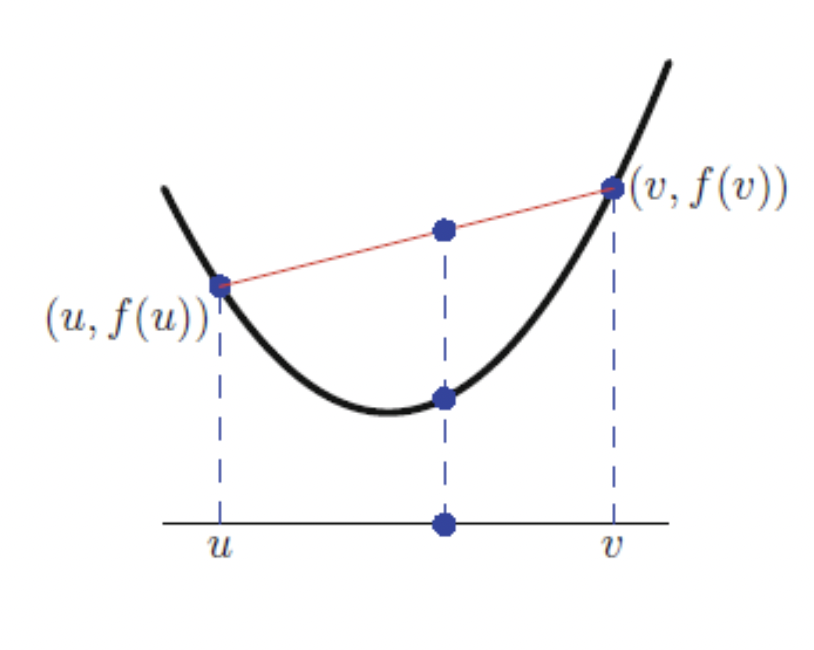
\includegraphics[width=0.5\textwidth]{fig1.1.png}
	\\ Fig 1.1 Funcții convexe: graficul este sub coarda
\end{center}

Această remarcă arată faptul ca funcțiile convexe sunt majorate de funcțiile afine pe orice subinterval compact.

Orice funcție convexa f este marginită pe fiecare subinterval compact \(\left [ u , v \right ]\) al intervalului pe care este definită. De fapt , \(f\left ( x \right ) \leq  M = max \left \{ f\left ( u \right ), f\left ( v \right ) \right \}\)  pe \(\left [ u , v \right ]\)  și scriind acest lucru într-un punct arbitrar \(x\in  \left [ u , v  \right ]\)  de forma  \(x= \frac{\left ( u + v \right )}{2} + t\) pentru  \(t\) care verifică \(\left | t \right |\leq \frac{\left ( v - u \right )}{2}\), deducem cu usurința că

\begin{displaymath}
  f\left ( x \right )=  f\left ( \frac{u+v}{2} + t\right )\geq 2 f\left ( \frac{u + v}{2} \right )- f\left ( \frac{u + v}{2} - t\right )\geq 2f\left ( \frac{u+v}{2} \right ) - M.
\end{displaymath}

\begin{theorem}
O funcție convexă \(f: I \rightarrow \mathbb{R}\) este continuă în orice punct interior al lui \(I\). 	
\end{theorem}
\begin{proof}
	Presupunem că \(a\in I\) și alegem \(\varepsilon > 0\) astfel încat \(\left [ a - \varepsilon , a + \varepsilon  \right ] \subset I\).
 Atunci
\begin{displaymath}
  f\left ( a \right )\leq \frac{1}{2} f\left ( a - \varepsilon  \right ) + \frac{1}{2}f \left ( a + \varepsilon  \right )
\end{displaymath}
și
\begin{displaymath}
  f\left ( a \pm t\varepsilon  \right )= f\left ( \left ( 1 - t \right ) a + t\left ( a \pm \varepsilon  \right )\right )\leq \left ( 1 - t \right )f\left ( a \right ) + tf\left ( a\pm \varepsilon  \right )
\end{displaymath}
pentru orice \(t\in \left [ 0 , 1 \right ]\). Prin urmare
\begin{displaymath}
  t\left ( f\left ( a\pm \varepsilon  \right ) - f\left ( a \right ) \right )\geq f\left ( a\pm t\varepsilon  \right )- f\left ( a \right )\geq -t\left ( f\left ( a\mp \varepsilon  \right ) - f\left ( a \right )\right )
\end{displaymath}
care ne conduce la
\begin{displaymath}
\left | f\left ( a\pm t\varepsilon  \right )- f\left ( a \right ) \right |\leq t max \left \{ \left | f\left ( a-\varepsilon  \right )- f\left ( a \right ) \right |, \left | f\left ( a+\varepsilon  \right ) - f\left ( a \right )\right | \right \},
\end{displaymath}
 pentru orice \(t\in \left [ 0 , 1 \right ]\). Continuitatea funcției \(f\) este acum clară.
 \end{proof}

 \begin{remark}
	Exemple simple precum, \(f\left ( x \right )= 0\) dacă \(x\in \left ( 0 , 1 \right )\), și  \(f\left ( 0 \right )= f\left ( 1 \right ) = 1\), arată faptul că salturi  pot apărea în capetele intervalului de definiție al unei funcții convexe. Totuși, aceste posibile discontinuități pot fi înlăturate.
\end{remark}


\begin{proposition}
Dacă \(f: \left [ a, b \right ]\rightarrow \mathbb{R}\) este o funcție convexă, atunci limitele
\[
f\left ( a+ \right ) = \lim_{x\rightarrow a, x> a}f\left ( x \right ),~~ f\left ( b- \right ) = \lim_{x\rightarrow b, x< b}f\left ( x \right )\] există în \(\mathbb{R}\) și
\begin{displaymath}
  \tilde{f}\left ( x \right )= \left\{\begin{matrix}
f\left ( a+ \right ) & \\
 f\left ( x \right )& \\
 f\left ( b- \right )&
\end{matrix} \begin{matrix}
\text{dacă } x=a & \\
\text{dacă } x\in \left ( a,b \right ) & \\
\text{dacă } x= b&
\end{matrix}\right.
\end{displaymath}
 este o funcție convexă continuă.
\end{proposition}
	Acest rezultat este o consecință a următoarelor rezultate :
\begin{lemma}

Dacă \(f: I \rightarrow \mathbb{R}\) este convexă, atunci sau \(f\) este monotonă pe intervalul \(I\), sau există un punct \(\xi \in int I\) astfel încat \(f\) este descrescătoare pe intervalul \(\left ( -\infty , \xi  \right )\cap I\) și crescătoare pe intervalul \(\left[\xi , \infty  \right )\cap I\).
\end{lemma}
\begin{proof}
Luăm \(a < b\) puncte interioare arbitrare ale lui \(I\) și fie
\[m = inf\left \{ f\left ( x \right ): ~~x\in \left [ a,b \right ]\right \}.\] Cum \(f\) este continuă pe \(\left [ a,b \right ]\), acest infimum este atins în punctul \(\xi \in \left [ a,b \right ]\), adică
$
  m = f\left ( \xi  \right )
$
Dacă \(a \leq x <  y< \xi\), atunci \(y\) este o combinație convexă a lui \(x\) și \(\xi\), mai exact, \[y = \frac{\xi -y}{\xi -x}x + \frac{y - x}{\xi -x}\xi.\] Cum \(f\) este convexă,
\begin{displaymath}
  f\left ( y \right )\leq \frac{\xi -y}{\xi -x}f\left ( x \right )+ \frac{y-x}{\xi -x}f\left ( \xi  \right )\leq f\left ( x \right ).
\end{displaymath}
Demonstrația se incheie cu un proces de lipire (la stanga lui \(a\) și la dreapta lui \(b\)), observând că proprietatea de covexitate face imposibilă existența a trei numere \(u < v < w\) in \(I\) astfel încat \(f\left ( u \right ) < f\left ( v \right )> f\left ( w \right )\).
\end{proof}

\begin{corollary}
\begin{enumerate}[a)]
\item Orice funcție convexț \(f: I \rightarrow \mathbb{R}\) care nu este monotonă pe
intervalul \(I\) are un minim global interior.
\item Dacă o funcție convexă \(f: \mathbb{R} \rightarrow \mathbb{R}\) este marginită superior, atunci este constantă.
\end{enumerate}
\end{corollary}
Atingere supremului la capete nu este o proprietate caracteristică a funcțiilor convexe, dar avem însă urmatorul rezultat.

\begin{theorem}

Fie \(f: I \rightarrow \mathbb{R}\). Atunci \(f\) este (strict) convexă daca și numai dacă pentru orice subinterval compact \(J\) al lui \(I\), și fiecare funcție afină \(L\), supremul lui \(f+L\) pe \(J\) este atins într-un capăt al intervalului (și doar acolo).
\end{theorem}

\begin{proof}
Ne vom restrange la cazul funcțiilor convexe. Cazul funcțiilor strict convexe poate fi tratat în acelasi mod.

\textbf{Necesitatea:} Dacă \(f\) este convexă, la fel este și suma \(F = f + L\). Cum orice punct al unui subinterval \(J = \left [ x , y \right ]\) este o combinație convexă \(z = \left ( 1 - \lambda  \right )x + \lambda y \) a lui \(x\) și \(y\), avem
\begin{equation*}
\begin{split}
  \sup_{z\in J}F\left ( z \right ) &= \sup_{\lambda \in \left [ 0 , 1 \right ]}F\left ( \left ( 1 - \lambda  \right )x + \lambda y \right )\\
  &\leq \sup_{\lambda \in \left [ 0,1 \right ]}\left [ \left ( 1-\lambda  \right )F\left ( x \right ) + \lambda F\left ( y \right ) \right ] + max \left \{ F\left ( x \right ), F\left ( y \right ) \right \}
  \end{split}
\end{equation*}

\textbf{Suficiența:} Având un subinterval \(J = \left [ x,y \right ]\) al lui \(I\), există o funcție afină \(L\left ( x \right ) = mx + n\) care este egală cu \(f\) în cele doua puncte  \(x\) si \(y\).
Atunci
\begin{displaymath}
  \sup_{\lambda \in \left [ 0,1 \right ]}\left [ \left ( f - L \right )\left ( 1 - \lambda  \right )x + \lambda y \right ] = 0,
\end{displaymath}
care ne conduce la
\begin{displaymath}
  0\geq f\left ( \left ( 1 - \lambda  \right )x + \lambda y \right )- L\left ( \left ( 1 - \lambda  \right )x - \lambda L \right )
\end{displaymath}
  \begin{displaymath}
  = f\left ( \left ( 1 - \lambda  \right )x + \lambda y  \right ) - \left ( 1 - \lambda  \right )L\left ( x \right ) - \lambda L\left ( y \right )
\end{displaymath}
\begin{displaymath}
  = f\left ( \left ( 1 - \lambda  \right )x + \lambda y \right ) - \left ( 1 - \lambda  \right ) f\left ( x \right ) - \lambda f \left ( y \right ),
\end{displaymath}
pentru orice \(\lambda \in \left [ 0,1 \right ]\).
\end{proof}

\begin{definition}
O funcție \(f: I \rightarrow \mathbb{R}\) se numește cvasiconvexă dacă,
 \begin{displaymath}
  f\left ( \left ( 1-\lambda  \right )x + \lambda y \right )\geq  min\left \{ f\left ( x \right ), f\left ( y \right ) \right \}
\end{displaymath}
pentru orice  \(x, y \in I\) și \(\lambda  \in \left ( 0,1 \right ]\).
\end{definition}
	 Avem următoarea caracterizare a convexității în cadrul clasei funcțiilor continue care se dovedește utilă și în verificarea convexității.
\begin{theorem}
O funcție \(f : I \rightarrow \mathbb{R}\) este convexă dacă și numai dacă ea verifică urmatoarele două condiții:
\begin{enumerate}[a)]
\item \(f\) este continuă în fiecare punct din interiorul lui \(I\); și
\item \(f\) este convexă în punctul de mijloc , adică,
\end{enumerate}
\begin{displaymath}
  f\left ( \frac{x+y}{2} \right )\leq \frac{f\left ( x \right )+f\left ( y \right )}{2}, \text{ pentru orice } x, y \in I.
\end{displaymath}
\end{theorem}
\begin{proof}
\textbf{Necesitatea }rezultă din teorema 1.1.2.

\textbf{Suficiența} o vom demonstra prin reducere la absurd. Dacă \(f\) nu este convexă, atunci există un interval \(\left [ a,b \right ]\) astfel încat graficul funcției \(f\) restricționată la  \(\left [ a,b \right ]\) să nu fie sub coarda care unește punctele \(\left ( a, f\left ( a \right ) \right )\) și \(\left ( b, f\left ( b \right ) \right )\); ca urmare , funcția
\begin{displaymath}
  \varphi \left ( x \right )= -f\left ( x \right ) + f\left ( a \right )+ \frac{f\left ( b \right )- f\left ( a \right )}{b-a}\left ( x-a \right ), x\in \left [ a,b \right ]
\end{displaymath}
are  \(\gamma = inf \left \{ \varphi \left ( x \right ) : x\in \left [ a,b \right ]\right \}< 0\).

Observam că \(-\varphi\) este convexă în punctul de mijloc, continuă și \(\varphi \left ( a \right ) =\varphi \left ( b \right ) = 0\). Fie \(c = inf \left \{ x \in \left [ a,b  \right ] : \varphi \left ( x \right )= \gamma \right \} \), atunci \(\varphi \left ( c \right ) = \gamma\)  și \(c \in \left ( a,b  \right )\). Conform definiției lui \(c\), pentru orice \(h>0\) pentru care \(c\pm h\in \left ( a,b \right )\) avem
\begin{displaymath}
  \varphi \left ( c - h  \right )> \varphi \left ( c \right ) si \varphi \left ( c + h  \right )\geq  \varphi \left ( c \right )
\end{displaymath}

Astfel
\begin{displaymath}
  -\varphi \left ( c \right )> \frac{-\varphi \left ( c-h \right )-\varphi \left ( c+h \right )}{2},
\end{displaymath}
ceea ce este în contradicție cu faptul că \(-\varphi\) este convexă în punctul de mijloc.
\end{proof}


\begin{corollary}
Fie \(f: I \rightarrow \mathbb{R}\) o funcție continuă. Atunci, \(f\) este convexă daca și numai dacă
\begin{displaymath}
  f\left ( x+h \right )+ f\left ( x - h \right ) - 2f\left ( x \right )\geq 0
\end{displaymath}
pentru orice \(x \in I\) și orice \(h > 0\) astfel încat și \(x + h\) și \(x - h\) aparțin lui \(I\).
\end{corollary}
\begin{remark}
Observăm că și Teorema 1.1.8 și Corolarul acesteia 1.1.9 de mai sus, admit variante în cazul funcțiilor strict convexe,
Corolarul 1.1.9 ne permite să verificăm imedat convexitatea / concavitatea strictă a unor funcții elementare, precum funcția exponențială, cea logaritmică, și restricția funcției sinus pe \(\left [ 0 , \pi \right ]\).

Într-adevar, pentru funcția exponențială, faptul că  \(a , b > 0, a\neq b\), implica \(\frac{a + b}{2}> \sqrt{ab}\)
este echivalentă cu
\(e^{x + h} + e^{x - h } - 2e^{x}> 0\)
pentru orice \(x\in \mathbb{R}\) și orice \(h > 0\).
\end{remark}
	Multe alte exemple pot fi deduse folosind următoarele proprietăți ale funcțiilor convexe / concave.

\begin{proposition}
\textbf{Operații cu funcții convexe:}
\begin{enumerate}[a)]
\item Adunând două funcții convexe ( definite pe același interval) obținem o funcție convexă; dacă una dintre ele este strict convexă, atunci suma lor este de asemenea strict convexă.
\item Înmulțind o funcție (strict) convexă cu un scalar (strict)  pozitiv obținem de asemenea o funcție (strict) convexă.
\item Presupunem că f și g sunt două funcții convexe pozitive definite pe un interval I. Atunci, produsul lor este o funcție convexă pe I dacă sunt sincrone în sensul că, \begin{displaymath}
   \left ( f\left ( x \right ) - f\left ( y \right ) \right )\left ( g\left ( x \right ) - g\left ( y \right )\right )\geq 0
\end{displaymath} pentru orice \(x , y \in \mathbb{R}\); de exemplu , această condiție apare daca f și g sunt amandouă descrescătoare sau amândouă crescătoare.
\item Restricția unei funcții (strict) convexe pe I, la un subinterval al lui I este de asemenea o funcție (strict) convexă.
\item Presupunem că \(f\) este o funcție bijectivă între două intervale \(I\) si \(J\). Dacă \(f\) este strict crescătoare, atunci \(f\) este (strict) convexă dacă și numai dacă \(f^{-1}\) este (strict) concavă. Dacă \(f\) este o funcție bijectivă descrescătoare, atunci \(f\) și  \(f^{-1}\) sunt ambele convexe sau ambele concave.
\item Dacă \(f\) este o funcție strict pozitivă concavă, atunci \(\frac{1}{f}\) este o funcție convexă. Aici rolul concavității și al convexității nu poate fi schimbat unul cu celălalt.
\item Maximul a doua funcții (stricte) convexe \(f , g : I \rightarrow \mathbb{R}\),
\begin{displaymath}
  max \left \{ f , g \right \}\left ( x \right )=  max \left \{ f\left ( x \right ), g\left ( x \right ) \right \}
\end{displaymath} este de asemenea o funcție (strict) convexă.
\item Compunerea \(f\left ( ax + b \right )\), a unei funcții \(f\) convexe și a unei funcții afine \(ax+b\), este o funcție convexă.
\end{enumerate}
\end{proposition}
În continuare, vom discuta extinderea inegalității convexității (1.1). În primul rand, observăm faptul că intervalele sunt închise la combinații convexe arbitrare, adică,
\begin{displaymath}
  \sum_{ k= 1}^{n}\lambda _{k}x_{k} \in I~~\mbox{pentru orice}~~x_{1},\cdots, x_{n} \in I  ~~\mbox{și orice}~~\lambda _{1},\cdots, \lambda _{n} \in \left [ 0 , 1  \right ]
\end{displaymath}
 cu \(\sum_{k = 1}^{n} \lambda _{k} = 1\).

 Acest lucru poate fi demonstrat prin inducție după \(n\).

 Cazul \(n=1\) este trivial, în timp ce \(n = 2\) rezultă din definiția unei mulțimi convexe.

  Presupunând faptul că rezultatul este adevărat pentru toate combinațiile convexe cu cel mult \(n\geq 2\) puncte, să trecem la cazul combinațiilor cu \(n + 1\) puncte, \(x = \sum_{k = 1}^{n + 1} \lambda _{k}x_{k}\). Cazul non-trivial este atunci cand toți coeficienții \(\lambda _{k}\) se află în \(\left ( 0 , 1 \right )\). Dar în acest caz, datorită ipotezei de inducție, x poate fi reprezentat ca o combinație convexă de doua elemente ale lui \(I\),
\begin{displaymath}
  x = \left ( 1 - \lambda _{n + 1} \right )\left ( \sum_{k = 1}^{n} \frac{\lambda _{k}}{1 - \lambda _{n + 1}} x_{k}\right ) + \lambda _{n + 1}x_{n + 1},
\end{displaymath}
prin urmare x apartine lui \(I\).
	Observația de mai sus asupra intervalelor are o echivalență remarcabilă pentru funcțiile convexe:

\begin{lemma}
\textbf{Cazul discret al inegalității lui Jensen}

O funcție cu valori reale \(f\) definită pe un interval \(I\) este convexă dacă și numai dacă pentru orice puncte \(x_{1},\cdots,x_{n}\) din \(I\) și orice scalari \(\lambda _{1},\cdots,\lambda _{n}\) din \(\left [ 0 , 1 \right ]\) cu \(\sum_{k = 1}^{n}\lambda _{k}= 1\) avem,
\begin{displaymath}
  f\left ( \sum_{k = 1}^{n} \lambda _{k}x_{k}\right )\leq \sum_{k = 1}^{n}\lambda _{k}f\left ( x_{k} \right ).
\end{displaymath}

Dacă \(f\) este strict convexă, inegalitatea de mai sus este strictă dacă punctele \(x_{k}\) nu sunt toate egale între ele , și scalarii \(\lambda _{k}\) sunt toți pozitivi.
\end{lemma}
\begin{proof}
Prima afirmație rezultă prin inducție matematică.

În ceea ce privește cea de a doua afirmație, presupunem că funcția \(f\) este strict convexă și
\begin{displaymath}
  f\left ( \sum_{k = 1}^{n} \lambda _{k}x_{k}\right )=  \sum_{k = 1}^{n}\lambda _{k}f\left ( x_{k} \right ). \label{eq:1.3} \tag{1.3}
\end{displaymath}
pentru  punctele \(x_{1}, \cdots, x_{n} \in I\) și scalarii \(\lambda _{1}, \cdots, \lambda _{n} \in \left ( 0 , 1\right )\) care au suma egala cu \(1\). Dacă \(x_{1}, \cdots, x_{n}\) nu sunt toți egali, mulțimea
\[S = \left \{ k: x_{k}<  max \left \{ x_{1,\cdots,x_{n}} \right \} \right \}\]
 va fi o submulțime proprie a mulțimii  \(\left \{ 1,\cdots,n \right \}\) și \(\lambda _{S} = \sum_{k \in S}^{}\lambda _{S} \in \left ( 0,1 \right )\). Cum \(f\) este strict convexă avem,
\begin{displaymath}
  f\left ( \sum_{k=1}^{n}\lambda _{k}x_{k} \right ) = f\left ( \lambda _{S}\left ( \sum_{k\in S}^{}\frac{\lambda _{k}}{\lambda _{S}} x_{k}\right ) +\left ( 1-\lambda _{S} \right )\left ( \sum_{k\notin S}^{} \frac{\lambda _{k}}{1 - \lambda _{S}}x_{k}\right )\right ) <
\end{displaymath}
\begin{displaymath}
  \lambda _{S}f\left ( \sum_{k\in S}^{}\frac{\lambda _{k}}{\lambda _{S}} x_{k}\right ) +\left ( 1 - \lambda _{S} \right )f\left ( \sum_{k\notin S}^{}\frac{\lambda _{k}}{1 - \lambda _{S}} x_{k}\right ) <
\end{displaymath}

\begin{displaymath}
  \lambda _{S} \sum_{k\in S}^{}\frac{\lambda _{k}}{\lambda _{S}} f\left ( x_{k} \right ) +\left ( 1 - \lambda _{S} \right ) \sum_{k\notin S}^{}\frac{\lambda _{k}}{1 - \lambda _{S}}f\left ( x_{k} \right )= \sum_{k=1}^{n}\lambda _{k}f\left ( x_{k} \right ),
\end{displaymath}
care contrazice ipoteza noastră \ref{eq:1.3}. Astfel, toate punctele \(x_{k}\) ar trebui să coincidă.
\end{proof}

O consecință imediată a lemei 1.1.11 (când este aplicată funcției exponențiale) este urmatorul rezultat care extinde bine cunoscuta inegalitate MA-MG (adica inegalitatea dintre media aritmetică și cea geometrică).


\begin{theorem}
\textbf{Forma ponderată a inegaliățtii mediilor}

Dacă \(x_{1},\cdots,x_{n}\in \left ( 0,\infty  \right ) si \lambda_{1},\cdots,\lambda _{n} \in \left ( 0 , 1 \right ), \sum_{k = 1}^{n}\lambda _{k}= 1\), atunci
\begin{displaymath}
  \sum_{k = 1}^{n}\lambda _{k}x_{k}> x_{1}^{\lambda _{1}}\cdots x_{n}^{\lambda _{n}}
\end{displaymath}
în afară de cazul când \(x_{1} = \cdots = x_{n}\).
	
	Înlocuind \(x_{k}\) cu \(\frac{1}{x_{k} }\) în ultima inegalitate, obținem
\begin{displaymath}
  x_{1}^{\lambda _{1}}\cdots x_{n}^{\lambda _{n}}> \frac{1}{\sum_{k = 1}^{n}\lambda _{k}\frac{1}{x_{k}}}
\end{displaymath}
în afară de cazul când \(x_{1} = \cdots = x_{n}\).
\end{theorem}
Aceasta reprezintă forma ponderată a inegalității mediei geometrice – mediei armonice (adica inegalitatea MG-MH).

Pentru \(\lambda _{1} = \cdots =\lambda _{n}= \frac{1}{n}\) obținem inegalitatea obișnuită care afirmă că pentru orice \(x_{1},\cdots,x_{n}\)  numere pozitive, nu toate egale, avem

\begin{displaymath}
  \frac{x_{1}+\cdots+x_{n}}{n}> \sqrt[n]{x_{1}\cdots x_{n}}> \frac{n}{\left ( \frac{1}{x_{1}}+\cdots+\frac{1}{x_{n}} \right )}.
\end{displaymath}




\section{Inegalitatea lui Young și consecințele sale}

Următoarul caz special al formei ponderate a inegalității MA-MG este cunoscută sub numele de inegalitatea lui Young:
\begin{displaymath}
  ab \leq \frac{a^{p}}{p}+ \frac{b^{q}}{q},
\end{displaymath}
pentru orice \(a,b \geq 0\)
și pentru orice  \(p,q \in \left ( 0 , 1 \right )\) cu proprietatea că \(\frac{1}{p}+\frac{1}{q} = 1\).
Egalitatea are loc dacă și numai dacă \(a^{p}= b^{q}\).

Inegalitatea lui Young poate fi de asemenea obținută ca o consecină a convexității stricte a funcției exponențiale.

Într-adevar
\begin{displaymath}
  ab = e^{\log_{a}b}= e^{\left (\frac{1}{p}  \right )\log_{a}p+ \left ( \frac{1}{q} \right )\log_{b}q}
< \frac{1}{p}e^{\log_{a}p}+\frac{1}{q}e^{\log_{b}q}= \frac{a^{p}}{p}+\frac{b^{q}}{q},
\end{displaymath}
pentru orice \(a,b>0\) astfel incat \(a^{p}\neq b^{q}\).

O altă soluție este oferită de studiul variației funcției diferențiabile
\begin{displaymath}
  F\left ( a \right )= \frac{a^{p}}{p}+\frac{b^{q}}{q} - ab,~ a\geq 0,
\end{displaymath}
unde \(b\geq 0\) este un paramentru. Această funcție iși atinge punctul de minim global strict în \(a= b^{\frac{q}{p}}\), care ne conduce la \(F\left ( a \right )> F\left ( b^{\frac{q}{p}} \right ) = 0\) pentru orice \(a\geq 0, a\neq b^{\frac{q}{p}}\).

	W.H.Young a dovedid de fapt  o inegalitate mult mai generală, pentru \(f\left ( x \right )=  x^{p-1}\).

\begin{theorem}
\textbf{Inegalitatea lui Young
}
Presupunem că \(f: \left [ 0,\infty  \right ) \rightarrow \left [ 0,\infty  \right )\) este o funcție continuă strict crescătoare astfel încat \(f\left ( 0 \right )= 0\) si \(\lim_{x\rightarrow \infty }f\left ( x \right )= \infty\). Atunci
\begin{displaymath}
  uv\leq \int_{0}^{u}f\left ( x \right )dx + \int_{0}^{v}f^{-1}\left ( y \right )dy
\end{displaymath}
pentru orice \(u,v\geq 0\) cu egalitate dacă și numai dacă \( v = f\left ( u \right )\).
\end{theorem}
\begin{center}
	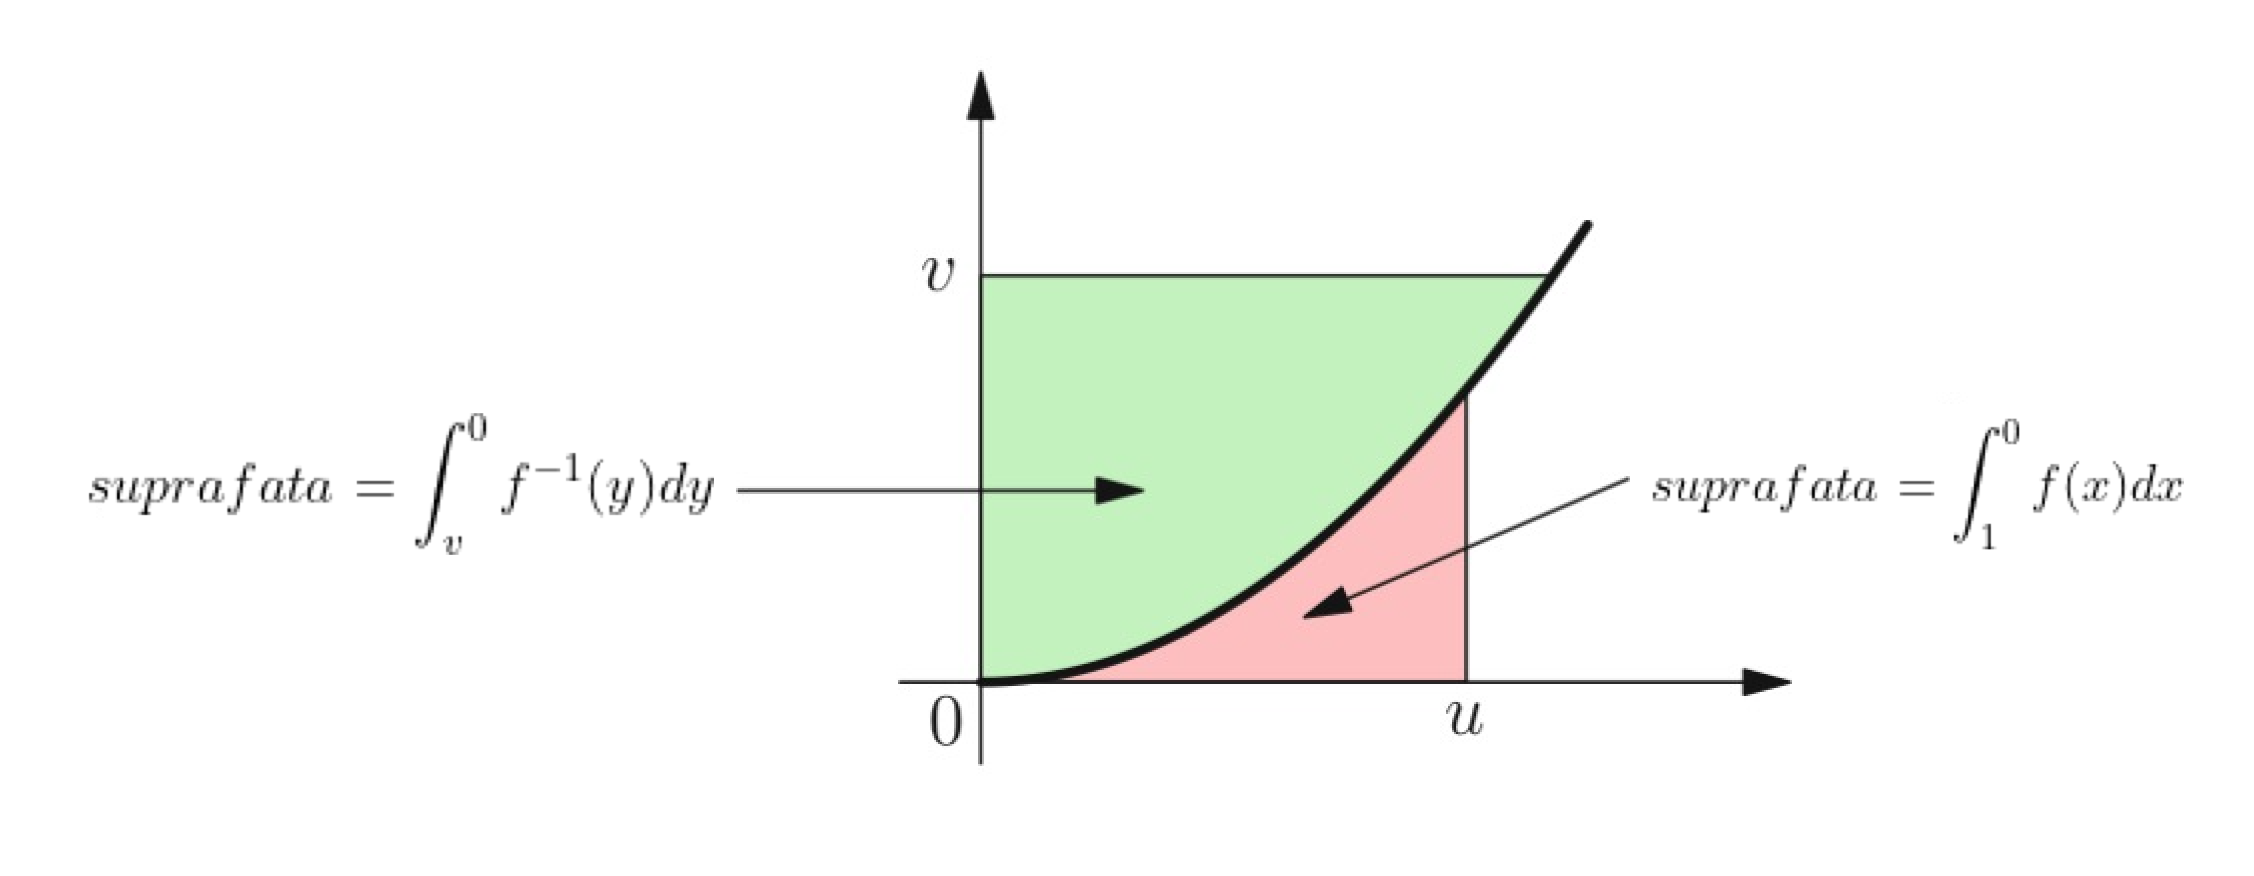
\includegraphics[width=1.0\textwidth]{fig1.2.png}
	\\ Fig 1.2 Aria  de unire a celor doua triunghiuri curbilinii depășește aria dreptunghiului cu laturile u si v
\end{center}

\begin{proof}
Folosind definiția derivatei se poate demonstra cu usurință că funcția
\begin{displaymath}
  F\left ( u \right )= \int_{0}^{u}f\left ( x \right )dx + \int_{0}^{f\left ( u \right )}f^{-1}\left ( y \right )dy -uf\left ( u \right ), u \in \left [ 0,\infty  \right )
\end{displaymath}
este diferențiabilă, cu \({F}'\) $\equiv 0.$ Astfel, \(F\left ( u \right )= F\left ( 0 \right )= 0\) pentru orice \(u\geq 0\).
	
Dacă \(u, v \geq 0\)  si \(v\geq f\left ( u \right )\), atunci
\begin{displaymath}
  uv = uf\left ( u \right )+ u\left ( v- f\left ( u \right ) \right )=  \int_{0}^{u}f\left ( x \right )dx + \int_{0}^{f\left ( u \right )}f^{-1}\left ( y \right )dy + u\left ( v - f\left ( u \right ) \right ) =
\end{displaymath}

\begin{displaymath}
  = \int_{0}^{u}f\left ( x \right )dx + \int_{0}^{v}f^{-1}\left ( y \right )dy + \left [ u\left ( v-f\left ( u \right )  \right ) - \int_{f\left ( u \right )}^{v}f^{-1}\left ( y \right )dy\right ]\leq
\end{displaymath}

\begin{displaymath}
  \leq \int_{0}^{u}f\left ( x \right )dx + \int_{0}^{v}f^{-1}\left ( y \right )dy.
\end{displaymath}



	Celălalt caz, unde \(v\leq f\left ( u \right )\) poate fi tratat similar.
\end{proof}

\begin{theorem}

\textbf{Inegalitatea lui Rogers-Hölder pentru} \(p > 1\)

Fie \(p,q \in \left ( 1, \infty  \right )\) cu \(\frac{1}{p} + \frac{1}{q} = 1\) si  \(f\in L^{p}\left ( \mu  \right )\) si \(g\in L^{q}\left ( \mu  \right )\). Atunci \(fg\) aparține lui \(L^{1}\left ( \mu  \right )\) si avem
\begin{displaymath}
  \left | \int_{\Omega}^{} fg  d\mu \right |\leq \int_{\Omega}^{}\left | fg \right |d\mu \label{eq:1.6} \tag{1.6}
\end{displaymath}
și
\begin{displaymath}
  \int_{\Omega}^{}\left | fg \right |d\mu \leq \left \| f \right \|_{L^{p}}\left \| g \right \|_{{L}^{q}}. \label{eq:1.7} \tag{1.7}
\end{displaymath}
Ca o consecință
\begin{displaymath}
  \left | \int_{\Omega}^{} fg  d\mu \right |\leq \left \| f \right \|_{L^{p}}\left \| g \right \|_{{L}^{q}}. \label{eq:1.8} \tag{1.8}
\end{displaymath}
\end{theorem}

\begin{remark}
	Rezultatul de mai sus se extinde într-o maniera directă la perechi de forma \(p = 1, q = \infty\) și \(p = \infty, q = 1\).
	
Din Inegalitatea Rogers – Hölder rezultă că pentru orice \(p, q, r \in \left ( 1 , \infty  \right )\) cu \(\frac{1}{p} + \frac{1}{q} = 1\) și orice \(f\in L^{p}\left ( \mu  \right )\) si \(g\in L^{q}\left ( \mu  \right )\) avem \(fg\in L^{r}\left ( \mu  \right )\) și
\begin{displaymath}
  \left \| fg \right \|_{L^{r}}\leq \left \| f \right \|_{L^{p}}\left \| g \right \|_{L^{q}} \label{eq:1.9} \tag{1.9}
\end{displaymath}


Inegalitatea \ref{eq:1.8}, pentru \(p = q = 2\), este cunoscută ca \textbf{inegalitatea Cauchy-Bunyakovsky-Schwarz} pentru integrale.
\end{remark}
\begin{proof}
Prima inegalitate este trivială.

Dacă \(f\) sau \(g\) sunt \(0~~ \mu\) – aproape peste tot, atunci cea de a doua inegalitate este trivială. Altfel, folosind inegalitatea lui Young, avem
\begin{displaymath}
  \frac{\left | f\left ( x \right ) \right |}{\left \| f \right \|_{L^{p}}} \cdot \frac{\left | g\left ( x \right ) \right |}{\left \| g \right \|_{L^{q}}}\leq \frac{1}{p}\cdot \frac{\left | f\left ( x \right ) \right |^{p}}{\left \| f \right \|^{p}_{L^{p}}} + \frac{1}{q}\cdot \frac{\left | g\left ( x \right ) \right |^{q}}{\left \| g \right \|^{q}_{L^{q}}}
\end{displaymath}
 pentru orice \(x\) din \(\Omega\). Astfel deducem că \(fg \in L^{1}\left ( \mu  \right )\). De asemenea
\begin{displaymath}
  \frac{1}{\left \| f \right \|_{L^{p}}\left \| g \right \|_{L^{q}}}\int_{\Omega }\left | fg \right |d\mu \leq 1.
\end{displaymath}
\end{proof}

\begin{remark}

Condiții pentru egalitatea din Teorma 1.2.2

Observația de bază este faptul că  \(f\geq 0\) si \(\int_{\Omega }f d\mu  = 0\) implică \(f = 0~~ \mu-\) aproape peste tot.
	Prin urmare avem egalitate in \ref{eq:1.6} dacă și numai dacă
\begin{displaymath}
  f\left ( x \right )g\left ( x \right ) = e^{i\theta }\left | f\left ( x \right ) g\left ( x \right )\right |
\end{displaymath}
pentru o constantă reală \(\theta\) și pentru \(\mu-\) aproape peste toți \(x\).


	Presupunem că \(p , q \in \left ( 1 , \infty  \right )\) și \(f\) si \(g\) nu sunt zero \(\mu-\) aproape peste tot. Pentru a avea egalitate in \ref{eq:1.7} este necesar și suficient să avem
\begin{displaymath}
  \frac{\left | f\left ( x \right ) \right |}{\left \| f \right \|_{L^{p}}} \cdot \frac{\left | g\left ( x \right ) \right |}{\left \| g \right \|_{L^{q}}}\leq \frac{1}{p}\cdot \frac{\left | f\left ( x \right ) \right |^{p}}{\left \| f \right \|^{p}_{L^{p}}} + \frac{1}{q}\cdot \frac{\left | g\left ( x \right ) \right |^{q}}{\left \| g \right \|^{q}_{L^{q}}}
\end{displaymath}

\(\mu-~\)aproape peste tot.

Cazul egalității în Inegalitatea lui Young demonstrează că aceasta este echivalentă cu \(A\left | f\left ( x \right ) \right |^{p} = B\left | g\left ( x \right ) \right |^{q}~~ \mu-\)aproape peste tot,
unde A și B sunt două constante pozitive.

	Dacă \(p = 1\) si \(q = \infty\), avem egalitate în ecuația \ref{eq:1.7} dacă și numai dacă există o constantă \(\lambda \geq 0\) astfel încat \(\left | g\left ( x \right ) \right |\leq \lambda\),  \(\mu\) aproape peste tot și \(\left | g\left ( x \right ) \right |= \lambda,  \mu\) aproape peste tot pe mulțimea \(\left \{ x : f\left ( x \right )\neq 0 \right \}\).
\end{remark}
\begin{theorem}
\textbf{Inegalitatea Minkowski}\\

Pentru \(1\leq  p < \infty\) si \(f , g \in L^{p}\left ( \mu  \right ) \) avem
\begin{displaymath}
  \left \| f + g  \right \|_{L^{p}}\leq \left \| f \right \|_{L^{p}} + \left \| g \right \|_{L^{p}}. \label{eq:1.10} \tag{1.10}
\end{displaymath}
\end{theorem}
\begin{proof}
Pentru \(p  = 1\), inegalitatea \ref{eq:1.10} rezulta imediat prin integrarea inegalitatii \(\left | f + g \right |\leq \left | f \right | + \left | g \right |\).

Pentru \(p \in \left ( 1 , \infty  \right )\) avem:
\begin{displaymath}
  \left | f + g  \right |^{p}\leq \left ( \left | f \right | +\left | g \right |\right )^{p}\leq \left ( 2 \sup\left \{ \left | f \right |,\left | g \right | \right \} \right )^{p}\leq 2^{p}\left ( \left | f \right |^{p}  + \left | g \right |^{p}\right )
\end{displaymath}
care ne demonstrează că \(f + g \in L^{p}\left ( \mu  \right )\). Mai mult de atât, conform Teoremei 1.2.2,
\begin{displaymath}
  \left \| f + g  \right \|_{L^{p}}^{p} = \int_{\Omega }\left | f + g \right |^{p}d\mu \leq \int_{\Omega }\left | f + g \right |^{p - 1}\left | f \right |d\mu + \int_{\Omega }\left | f + g  \right |^{p - 1}\left | g \right |d\mu \leq
\end{displaymath}
\begin{displaymath}
  \leq\left ( \int_{\Omega }\left | f \right |^{p}d\mu  \right )^{\frac{1}{p}}\left ( \int_{\Omega }\left | f + g  \right | ^{\left ( p - 1 \right )}d\mu \right )^{\frac{1}{q}}+ \left ( \int_{\Omega }\left | g \right |^{p}d\mu  \right )^{\frac{1}{p}}\left ( \int_{\Omega} \left | f + g \right |^{\left ( p - 1 \right )q}d\mu \right )^{\frac{1}{q}}=
\end{displaymath}

\begin{displaymath}
  =\left ( \left \| f \right \|_{L^{p}} + \left \| g \right \|_{L^{p}} \right )\left \| f + g  \right \|_{L^{p}}^{\frac{p}{q}}
\end{displaymath}
unde \(\frac{1}{p} + \frac{1}{q} = 1\), deci avem că \(p - \frac{p}{q} = 1\). 	
\end{proof}



Dacă \(p = 1\), obținem egalitate în (1.10) dacă și numai dacă există o funcție masurabilă pozitivă \(\varphi\) astfel încât
\begin{displaymath}
  f\left ( x \right )\varphi \left ( x \right ) = g\left ( x \right )
\end{displaymath}
\(\mu –\) aproape peste tot pe multimea \(\left \{ x : f\left ( x \right )g\left ( x \right )\neq 0 \right \}\).

	Dacă \(p \in \left ( 1 , \infty  \right )\) și \(f\) nu este zero aproape peste tot, atunci avem egalitate în (1.10) dacă și numai dacă există  \(\lambda \geq 0\) constanta astfel încât \(g = \lambda f\) aproape peste tot.

	În  cazul particular în care \(\left ( \Omega , \Sigma, \mu \right )\) este spațiul cu masura asociat măsurii numărabile pe o mulțime finită, \[\mu  : \rho \left ( \left \{ 1,\cdots, n \right \} \right )\rightarrow \mathbb{N}, \mu \left ( A \right ) = \left | A \right |,\]
obținem formele clasice discrete ale inegalităților de mai sus.

De exemplu, poate fi obținută versiunea discretă a inegalității lui R\"{o}gers- Holder
\begin{displaymath}
  \left | \sum_{k=1}^{n} \xi _{k}\eta _{k}\right |\leq \left ( \sum_{k = 1}^{n}\left | \xi _{k}\right |^{p}  \right )^{\frac{1}{p}}\left ( \sum_{k = 1}^{n} \left | \eta _{k} \right |^{q}\right )^{\frac{1}{q}}
\end{displaymath}
pentru  orice \(\xi _{k}, \eta _{k} \in \left \{ 1,\cdots,n \right \}.\)




\textbf{Mai multe despre inegalitatea Cauchy – Bunyakovsky – Schwarz}

A.L. Cauchy , in faimosul sau curs de Analiză, folosind inegalitatea algebrica a  lui Lagrange
\begin{displaymath}
  \left ( \sum_{k = 1}^{n} a_{k}^{2}\right )\left ( \sum_{k = 1}^{n} b_{k}^{2}\right ) =  \sum_{1\leq j\leq k\leq n}\left ( a_{j}b_{k} - a_{k}b_{j} \right )^{2} + \left ( \sum_{k = 1}^{n} a_{k}b_{k}\right )^{2}
\end{displaymath}
a obținut cazul discret al inegalității Cauchy – Bunyakovsky – Schwarz
\begin{displaymath}
  \left | \sum_{k = 1}^{n} a_{k}b_{k} \right |\leq \left ( \sum_{k = 1}^{n}a_{k}^{2} \right )^{\frac{1}{2}}\left ( \sum_{k = 1}^{n}b_{k}^{2} \right )^{\frac{1}{2}}
\end{displaymath}
pentru orice numere reale \(a_{1},\cdots,a_{n}, b_{1},\cdots, b_{n}\). Cazul egalității este simplu de dedus.

Inegalitatea corespunzătoare pentru integrale a fost demonstrată independent de V. Y. Bunyakovsky și H.A.Schwarz.

	În 1890, H. Poincar\'{e} a observat versiunea integrală a identității algebrice a lui Lagrange (care conduce la inegalitatea Cauchy-Bunyakovsky-Schwarz în deplina sa generalitate):

Dacă \(\mu\) este o masură de probabilitate pe un spațiu \(\Omega\) si \(f\) si \(g\) sunt doua funcții aparținând spațiului \(L^{2}\left ( \mu  \right )\), atunci
\begin{displaymath}
\begin{split}
  \left (\int_{\Omega}f^{2}d\mu \right )\left (\int_{\Omega}g^{2}d\mu \right ) &- \left (\int_{\Omega}fgd\mu \right )^{2}\\
   &= \frac{1}{2}\int_{\Omega}\int_{\Omega}\left ( f\left ( x \right )g\left ( y \right ) - f\left ( y \right )g\left ( x \right )\right )^{2}d\mu \left ( x \right )d\mu \left ( y \right ).
  \end{split}
\end{displaymath}
	
	El a folosit această identitate integrală pentru a demonstra cazul unidimensional al unei inegalități care îi poartă numele. O altă demonstrație simplă a inegalității Cauchy-Bunyakovsky-Schwarz este oferită  de o identitate echivalentă cu legea cosinusurilor: pentru orice pereche de vectori nenuli \(x\) si \(y\) dintr-un spațiu vectorial real cu produs scalar, avem
\begin{displaymath}
  \left \| \frac{x}{\left \| x \right \|} - \frac{y}{\left \| y \right \|}\right \|^{2} = 2 - 2\frac{\left \langle x , y \right \rangle}{\left \| x \right \|\left \| y \right \|}.
\end{displaymath}

\section{Derivabilitatea func\c{t}iilor convexe}

Punctul de plecare este următoarea reformulare a definiției \ref{eq:1.1}. O funcție \(f : I \rightarrow \mathbb{R}\) este convexă dacă și numai dacă 
\begin{displaymath}
   f\left ( x \right ) \leq \frac{b - x}{b - a} \cdot f\left ( a \right ) + \frac{x- a}{b - a}f\left ( b \right ), \label{eq:1.11} \tag{1.11}
\end{displaymath}
ceea ce este echivalent cu 
\begin{displaymath}
   \begin{vmatrix}
1 &  a& f\left ( a \right )\\ 
 1&  x& f\left ( x \right )\\ 
 1&  b& f\left ( b \right )
\end{vmatrix} \geq 0, (1.12)
\label{eq:1.12} \tag{1.12}
\end{displaymath}
ori de câte ori \(a< x< b\) în I. Într-adevăr,  orice punct \(x\) care aparține unui interval \(\left [ a,b \right ]\) poate fi scris în mod unic, ca o combinație convexă a lui \(a\) și \(b\), mai precis,
\begin{displaymath}
    x = \frac{b - x}{b - a} \cdot a  + \frac{x- a}{b - a}\cdot b.
\end{displaymath}

Scăzând \(f\left ( a \right )\) din ambele părți ale inegalității \ref{eq:1.11} și repetând operația cu \(f\left ( b \right )\) în loc de \(f\left ( a \right )\), obținem faptul că orice funcție convexă \(f : I \rightarrow \mathbb{R}\) verifică teorema celor trei coarde, 
\begin{displaymath}
   \frac{f\left ( x \right ) - f\left ( a \right )}{x-a}\leq \frac{f\left ( b \right )- f\left ( a \right )}{b-a}\leq \frac{f\left ( b \right ) - f\left ( x \right )}{b-x} \label{eq:1.13} \tag{1.13}
\end{displaymath}
ori de câte ori \(< x< b\) în I, figura 1.3. În mod evient acestă inegalitate dapt caracterizează convexitatea lui f. Mai mult decât atât, inegalitatea celor trei coarde cu inegalitate strictă, ne oferă o caracterizare a convexității stricte. Foarte aproape de această observație este caracterizarea convexității , a lui Galvani .

Figgggggg


\begin{remark}
Inegalitatea celor trei coarde poate fi întărită după cum urmează : Dacă \((f : I \rightarrow \mathbb{R}\) este o funcție convexă , și \(x,y,a,b\) sunt puncte ale intervalului I astfel încât \(x \leq a, y\leq b, x \neq y\) și \(a \neq b\), atunci,
\end{remark}
\begin{displaymath}
   \frac{f\left ( x \right )- f\left ( y \right )}{x-y}\leq \frac{f\left ( a \right )- f\left ( b \right )}{a-b}. 
\end{displaymath}
\begin{theorem} \label{Teorema 7} \tag{Teorema 7}
Fie \(f : I \rightarrow \mathbb{R}\) o funcție convexă. Atunci \(f\) are are derivate finite la stânga și la dreapta fiecărui punct interior al lui I și \(x <y\) în intervalul I implică
\begin{displaymath}
   {f}'_{-}\left ( x \right )\leq {f}'_{+}\left ( x \right )\leq \frac{f\left ( y \right )-f\left ( x \right )}{y-x}\leq {f}'_{-}\left ( y \right )\leq {f}'_{+}\left ( x \right ).
\end{displaymath}
Mai mult, pe intervalul \(I, {f}'_{-}\) este continuă la stânga și \({f}'_{+}\) este continuă la dreapta. 
	Prin urmare , dacă o funcție convexă este diferențiabilă pe intervalul I, atunci aceasta este de asemenea continuu diferențiabilă. 
\end{theorem}
\begin{proof}
Într-adevăr , conform inegalității celor trei coarde, avem
\begin{displaymath}
   \frac{f\left ( x \right ) - f\left ( a \right )}{x-a} \leq \frac{f\left ( y \right ) - f\left ( a \right )}{y-a}\leq \frac{f\left ( z \right ) - f\left ( a \right )}{z -a }
\end{displaymath}
pentru orice \(x\leq y\leq a\leq z,\) din I. Acest lucru ne asigură faptul că există derivată la stânga în a și 
\begin{displaymath}
   {f}'_{-}\left ( a \right )\geq \frac{f\left ( z \right ) - f\left ( a \right )}{z-a}.
\end{displaymath}
Un argument simetric va da atunci existanța lui \({f}'_{+}\left ( a \right )\) existanța relației \({f}'_{-}\left ( a \right ) \leq  {f}'_{+}\left ( a \right )\). Pe de altă parte, începând cu \(x < u\leq v < y\) pe intervalul I, aceeași inegalitate a celor trei coarde ne conduce la
\begin{displaymath}
   \frac{f\left ( u \right ) - f\left ( x \right )}{u-x}\leq \frac{f\left ( v \right ) - f\left ( x \right )}{v - x}\leq \frac{f\left ( v \right ) - f\left ( y  \right )}{v - y},
\end{displaymath}
deci luând \(u\rightarrow x+\) și \(v\rightarrow y- \), obținem faptul că \({f}'_{+}\left ( x \right )\leq {f}'_{-}\left ( y \right ).\) 
Pentru continuitatea derivatelor unilaterale. Sî observăm că din continuitatea lui f pe intervalul I, deducem că 
\begin{displaymath}
   \frac{f\left ( y \right ) - f\left ( x \right )}{y-x} = \lim_{z \searrow x}\frac{f\left ( y \right ) - f\left ( z \right )}{y-z} \geq \lim_{z\searrow x}{f}'_{+}\left ( z \right )
\end{displaymath}
ori de câte ori \(x < z < y\). Trecând la limită, cum  \(y\searrow x \), obținem, 
\begin{displaymath}
 {f}'_{+}\left ( x \right ) \geq  \lim_{z \searrow x } {f}'_{+}\left ( z \right ). 
\end{displaymath}
Cum \({f}'_{+}\) este crescătoare, rămâne valabilă și inegalitatea inversă. Astfel, \({f}'_{+}\)  este drept continuă pe intervalul I. Continuitatea la stânga a lui \({f}'_{-}\)  poate fi demonstrată in mod similar. 
\end{proof}
Din teorema \ref{Teorema 7}, orice funcție convexă continuă \(f:\left [ a,b \right ]\rightarrow \mathbb{R}\) admite derivate unilaterale la capete, dar, pot fi infinite :
\begin{displaymath}
   - \infty  \leq  {f}'_{+}\left ( a \right ) \leq \infty
\end{displaymath}
și 
\begin{displaymath}
- \infty  \leq  {f}'_{-}\left ( b \right ) \leq \infty. 
\end{displaymath}
Această teoremă ne conduce de asemenea la faptul că p funcție convexă continuă \(f:\left [ a,b \right ]\rightarrow \mathbb{R}\) poate fi extinsă la o funcție convexă pe \(\mathbb{R}\) dacă și numai dacă   \({f}'_{+}\left ( a \right )\) și  \( {f}'_{-}\left ( b \right )\)  există și sunt finite. 

\textbf{Cât de ”nediferențiabilă” poate fi o funcție convexă ?}

Teorema \ref{Teorema 7} presupune faptul că orice funcție convexă \(f:I \rightarrow \mathbb{R}\) este derivabilă cu excepția unei mulțimi numărabile. De fapt, considerând mulțimea de nediferențiabilitate, 
\begin{displaymath}
   I_{nd} = \left \{ x : {f}'_{-}\left ( x \right )\leq {f}'_{+}\left ( x \right ) \right \}, 
\end{displaymath}
și alegând pentru orice \(x \in I_{nd}\) un punct rațional \(r_{x} \in \left ( {f}'_{-}\left ( x \right ),  {f}'_{+}\left ( x \right )  \right )\) vom avea o funcție identică \(\varphi : x \rightarrow r_{x}\) din \(I_{nd}\) către \(\mathbb{Q}\). Ca o consecință, \(I_{nd}\) este cel mult numrabilă. Să observăm faptul că acest raționament depinnde de axioma pe care o alegem. Un exemplu de funcție convexă pe \(\mathbb{R}\) pentru care \(I_{nd}\) este infinit numărabil este \(f\left ( x \right ) = \sum_{n = 0}^{\infty } \left | \frac{x-n}{2^{n}}\right |\). 

Teorema \ref{Teorema 7} ne oferă un argument alternativ pentru proprietatea funcțiilor convexe de a fi local Lipschitz pe intervalle deschise. Într-adevăr, dacă \(f : I \rightarrow \mathbb{R}\) este o funcție convexă și \(\left [ a,b \right ]\) este un interval compact din interiorul lui I, atunci 
\begin{displaymath}
   {f}'_{+}\left ( a \right ) \leq {f}'_{+}\left ( x \right )\leq \frac{f\left ( y \right )- f\left ( x \right )}{y-x}\leq  {f}'_{-}\left ( y \right )\leq {f}'_{-}\left ( b \right )
\end{displaymath}
pentru orice \(x,y \in \left [ a,b \right ]\), cu \(x< y\). Prin urmare \(f|_{\left | a,b \right |}\) verifică condiția Lipschitz \(\left | f\left ( x \right )  - f\left ( y \right )\right |\leq L\left | x-y \right |,\) cu \(L=\max \left \{ \left | {f}'_{+} \left ( a \right ),{f}'_{-} \left ( b \right ) \right | \right \}\). O consecință imediată este următorul rezultat :

\begin{theorem}
Dacă \(\left ( f_{n} \right )_{n}\) este o secvență convergentă punctuală de funcții convexe definite pe un interval deschis I, atunci limita sa f este de asemenea convexă. Mai mult, convergența este uniformă pe orice subinterval compact și 
\begin{displaymath}
   {f}'_{-}\left ( a \right ) \leq \lim_{n\rightarrow \infty } \inf {\left (f_{n}  \right )}'_{-}\left ( a \right )\leq \lim_{n\rightarrow \infty }\sup {\left (f_{n}  \right )}' + \left ( a \right ) \leq {f}'_{+}\left ( a \right ), pentru orice a \in I. 
\end{displaymath}
\end{theorem}
\begin{proof}
Convexitatea lui f este trivială. Din inegalitatea celor trei coarde (1.13), pentru orice \(h >  0\) cu \(a + h \in I\),
\begin{displaymath}
   {\left (f_{n}  \right )}'_{+}\left ( a \right ) \leq  \frac{f_{n}\left ( a + h \right ) - f_{n}\left ( a \right )}{h}
\end{displaymath}
astfel încât  
\begin{displaymath}
   \lim_{n\rightarrow \infty } \sup {\left ( f_{n} \right )}'_{+}\left ( a \right ) \leq \lim_{n\rightarrow \infty } \sup \frac{f_{n}\left ( a + h \right ) - f_{n}\left ( a \right )}{h} = \frac{f\left ( a + h \right ) - f\left ( a \right )}{h}. 
\end{displaymath}
Luân \(h\rightarrow 0\), obținem inegalitatea din partea dreaptă a teoremei 8. Inegalitatea din partea stângă poate fi demonstrată în mod similar. Ținând cont de o observație de mai sus despre Lipschitzianitatea locală a  funcțiilor convexe , se poate deduce cu ușurință convergența uniformă pe subintervale compacte ale lui I. 
\end{proof}
Este posibil, ca in egalitatea de mai sus, egalitatea să nu fie valabilă. Pentru a verifica asta, luăm în considerare succesiunea de funcții convexe \(f_{n}\left ( x \right ) = \left | x \right |^{1 + \frac{1}{n}}\) care converge pe \(\mathbb{R}\) către funcția \(f\left ( x  \right ) = \left | x \right |.\) Apoi, \({\left ( f_{n} \right )}'_{+}\left ( 0 \right ) = 0\) pentru orice \(n\) , în timp ce \({f}'_{+}\left ( 0 \right ) = 1.\) 

Următorul rezultat ne oferă o estimare superioară a inegalității lui Jensen :

\begin{theorem}
Fie \(f : \left [ a,b \right ] \rightarrow \mathbb{R}\) o funcție convexă și 
\begin{displaymath}
   \left [ m_{1}, M_{1} \right ],......,\left [ m_{n}, M_{n} \right ]
\end{displaymath}
subintervalele compacte ale lui \(\left [ a,b \right ]\). Luând \(\lambda _{1}, ....,\lambda _{n}\) în \(\left [ 0,1 \right ]\) cu \(\sum_{k = 1}^{n}\lambda _{k} = 1,\) funcția 
\begin{displaymath}
   E \left ( x_{1},....,x_{n} \right ) = \sum_{k = 1}^{n}\lambda _{k}f\left ( x_{k} \right ) - f\left ( \sum_{k=1}^{n}\lambda _{k}x_{k} \right ), 
\end{displaymath}
își atinge maximul în \(\Omega = \left [ m_{1}, M_{1} \right ] \times  \left [ m_{n}, M_{n} \right ] \)într-un vârf, adică într-un punct \(\left [ m_{1}, M_{1} \right ] \times\cdots \times   \left [ m_{n}, M_{n} \right ].\) 
\end{theorem}
Demonstrația depinde de următoarul rafinament al teoremei mediilor a lui Langrange :

\begin{lemma} \label{Lema 3} \tag{Lema 3}
Fie \(h : \left [ a,b\right ]\rightarrow \mathbb{R}\) o funcție continuă. Atunci există un punct \(c \in \left ( a,b \right )\) astfel încât 
\begin{displaymath}
   \underline{D}h\left ( c \right ) \leq  \frac{h\left ( b \right ) - h\left ( a \right )}{b-a}\leq \overline{D}h\left ( c \right ).
\end{displaymath}
Aici 
\begin{displaymath}
   \underline{\mathcal{D}}h\left ( c \right ) = \lim_{x\rightarrow c}  \frac{h\left ( x \right ) - h\left ( c \right )}{x-c} și \overline{\mathcal{D}}h\left ( c \right ) = \lim_{x\rightarrow c}  \frac{h\left ( x \right ) - h\left ( c \right )}{x-c}, 
\end{displaymath}
sunt, derivata inferioară respectiv derivata superioară a lui h în c. conform teoremei \ref{Teorema 7}, în cazul funcțiilor convexe , \(\overline{\mathcal{D}}h\left ( c \right ) = {h}'_{-}\left ( c \right )\)  și   \(\overline{\mathcal{D}}h\left ( c \right )  = {h}'_{+}\left ( c \right ).\) 
\end{lemma}
\begin{proof} Teorema 10
În mod clar, putem presupune faptul că f este de asemenea continuă. Vom demonstra ( prin reducere la absurd ) că
\begin{displaymath}
  E \left ( x_{1},....., x_{k},....x_{n} \right ) \leq  \sup \left \{ E\left ( x_{1},....,m_{k},....x_{n} \right ),E\left ( x_{1},....,M_{k},....x_{n} \right ) \right \},
\end{displaymath}
 pentru orice
\begin{displaymath}
     \left ( x_{1}, x_{2},....x_{n} \right ) \in\Omega, 
\end{displaymath}
și orice
\begin{displaymath}
    k \in\left \{ 1,....,n \right \}. 
\end{displaymath}
 De fapt, dacă
\begin{displaymath}
   E  \left ( x_{1}, x_{2},....x_{n} \right )  >  \sup \left \{ E\left ( m_{1}, x_{2} ,..., x_{n}\right ), E\left ( M_{1}, x_{2} ,..., x_{n}\right )  \right \}  
\end{displaymath}
pentru
\begin{displaymath}
  entru \left ( x_{1}, x_{2},....x_{n} \right ) \in \Omega,
\end{displaymath}
considerăm funcția 
\begin{displaymath}
  h : \left [ m_{1}, M_{1} \right ] \rightarrow \mathbb{R}, h\left ( x \right ) = E\left ( x_{1}, x_{2},...,x_{n} \right ). 
\end{displaymath}
Conform lemei \ref{Lema 3}, există \(\xi \in \left ( m_{1}, x_{1} \right )\) astfel încât \(h \left ( x_{1} \right ) - h\left ( m_{1} \right ) \leq  \left ( x_{1} - m_{1} \right )\overline{D}h\left ( \xi  \right ).\) 
Cum \(h \left ( x_{1} \right ) >  h\left ( m_{1} \right ),\) rezultă că \(\overline{D}h\left ( \xi  \right ) > 0\), ceea ce este echivalent cu 
\begin{displaymath}
   \overline{D}f\left ( \xi  \right ) > \overline{D}f\left (\lambda _{1}\xi +\lambda _{2}\xi +\cdots +\lambda _{n} x_{n} \right ). 
\end{displaymath}

Sau , \(\overline{D}f = {f}'_{+}\) este o funcție crecătoare pe \(\left ( a,b \right )\), ceea ce ne conduce la 
\begin{displaymath}
   \xi > \lambda _{1}\xi +\lambda _{2}x_{2} + \cdots +\lambda _{n}x_{n},
și atfel \xi = \frac{\lambda _{2}x_{2} + \cdots +\lambda _{n}x_{n}}{\lambda _{2}+\cdots +\lambda _{n}}.
\end{displaymath}
O nouă referire la lema \ref{Lema 3}( aplicată de data aceasta lui \(h|_{\left [ x_{1},M_{1} \right ]})\) ne conduce la existența unui \(\eta \in \left ( x_{1} , M_{1}\right )\) astfel încât \(\eta < \frac{\left ( \lambda _{2}x_{2}+\cdots +\lambda _{n}x_{n} \right )}{\lambda _{2}+\cdots +\lambda _{n}}\). Dar asta, contrazice faptul că \(\xi <  \eta \). 
\end{proof}
\begin{corollary} \label{Corolar 3} \tag{Corolar 3}
Fie \(f : \left [ a,b \right ] \rightarrow \mathbb{R}\) o funcție convexă. Atunci 
\begin{displaymath}
   \left ( 1-\lambda  \right )f\left ( a \right ) + \lambda f\left ( b \right ) - f\left ( \left ( 1-\lambda  \right )a + \lambda b \right )\geq \left ( 1-\lambda  \right )f\left ( c \right )+\lambda f\left ( d \right ) - f\left ( \left ( 1 -\lambda \right )c + \lambda d \right ), 
\end{displaymath}
pentru orice \(a\leq c\leq d\leq b \)și \(\lambda \in \left [ 0,1 \right ].\) 
\end{corollary}
Corolarul \ref{Corolar 3} este un prim pas către inegalitatea majorării. Din moment ce, derivata de ordin întâi a unei funcții convexe poate să nu existe  într-o submulțime densă, o caracterizare a convexității în termeni ai derivatei de ordinul doi nu este posibilă decât dacă relaxăm conceptul derivatei de ordinul doi. 

Derivatele, cea superioară și cea inferioară simetrică a derivatei lui f în x, sunt, definite de formulele
\begin{displaymath}
   \overline{ \mathcal{D}}^{2}f\left ( x \right ) = \lim_{h\downarrow0} \sup\frac{f\left ( x+h \right ) + f\left ( x-h \right ) -2f\left ( x \right )}{h^{2}}
\end{displaymath}
\begin{displaymath}
   \overline{ \mathcal{D}}^{2}f\left ( x \right ) = \lim_{h\downarrow0} \inf\frac{f\left ( x+h \right ) + f\left ( x-h \right ) -2f\left ( x \right )}{h^{2}}.
\end{displaymath}

Nu este greu să verificăm faptul că , dacă f este derivabilă de doua ori într-un punct x, atunci 
\begin{displaymath}
   \overline{ \mathcal{D}}^{2}f\left ( x \right ) = \underline{\mathcal{D}}^{2}f\left ( x \right ) = {f}''\left ( x \right ). \label{eq:1.14} \tag{eq1.14}
\end{displaymath}
totuși, \(\overline{ \mathcal{D}}^{2}f\left ( x \right )\) și \(\underline{\mathcal{D}}^{2}f\left ( x \right )\) pot exista chiar și la capetele de discontinuitate, de exemplu, să considerăm cazul funcției signum și puncul x = 0. Observațiade bază, pentru a demonstra relația \ref{eq:1.14}  este următoarea formulă
\begin{displaymath}
   f\left ( x + h \right ) - f\left ( x \right ) - h{f}'\left ( x \right ) - \frac{h^{2}}{2}{f}''\left ( x \right ) = o\left ( h^{2} \right ), 
\end{displaymath}
care se aplică pentru orice punct x în care f este derivabilă e două ori. Într-adevăr , arătând că partea stângă ca fiind \(g\left ( h \right )\), deducem din teorema mediilor faptul că \(g\left ( h \right ) = g \left ( h \right ) - g\left ( 0 \right ) = h{g}'\left ( k \right )\) și  \({g}'\left ( k \right ) = {g}'\left ( k \right ) - {g}'\left ( 0 \right ) = k{g}''\left ( 0 \right ) +o\left ( k \right ) = o\left ( k \right ). \)
	Prin urmare \(g\left ( h \right ) = ho\left ( k \right ) = o\left ( h^{2} \right ). \)
\begin{theorem}
Presupunem că I este un interval deschis. O funcție f cu valoare reală este convexă pe I dacă și numai dacă f este continuă și  \(\overline{ \mathcal{D}}^{2}f\geq 0.\) 
	Ca o consecință, dacă o funcție \(f : I \rightarrow \mathbb{R}\) este  funcție convexă  în vecinătatea fiecărui punct din I, atunci este convexă pe tot intervalul I. 
\end{theorem}
\begin{proof}
Dacă f este convexă, atunci, în mod clar \(\overline{ \mathcal{D}}^{2}f\geq \underline{\mathcal{D}}^{2}f\geq 0.\) Continuitatea lui f rezultă din teorema \ref{Teorema 7}. 

Acum, presupunem că \(\overline{ \mathcal{D}}^{2}f > 0\) pe I. Dacă f nu este convexă, atunci, utem găsi un punct \(x_{0}\), astfel încât \(\overline{ \mathcal{D}}^{2}f \left ( x_{0} \right )\geq 0\), ceea ce ar fi o contradicție. De fapt, în acest caz, există un subinterval \(I_{0} = \left [ a_{0}, b_{0} \right ]\) astfel încât \(f\left ( \frac{a_{0} + b_{0}}{2} \right )> \frac{f\left ( a_{0} \right ) + f\left ( b_{0} \right )}{2}.\) Dacă ne uităm cu atenție, observăm faptul că unul dintre intervale \(\left [ a_{0}, \frac{a_{0}+b_{0}}{2} \right ], \left [ \frac{\left ( 3a_{0}+b_{0} \right )}{4},\frac{\left ( a_{0}+3b_{0} \right )}{4} \right ],\left [\frac{a_{0}+b_{0}}{2}, b_{0} \right ]\) pot fi alese pentru a înlocui intervalul \(I_{0}\) cu un interval mai mic \(I_{1}= \left [ a_{1}, b_{1} \right ], cu  b_{1} -  a_{1}= \frac{b_{0}+ a_{0}}{2}\) și \(f\left ( \frac{a_{1}+b_{1}}{2} \right ) > \frac{f\left ( a_{1} \right ) + f\left ( b_{1} \right )}{2}.\) Cu ajutorul inducției, vom ajunge intr-o situație în care principiul intervalelor incluse o sa ne returneze punctul \(x_{0}.\)

În cazul general, considerăm urmatoare secvență de funcții 
\begin{displaymath}
   f_{n}\left ( x \right ) = f\left ( x \right ) + \frac{1}{n}x^{2}.
\end{displaymath}

Apoi, \(\overline{ \mathcal{D}}^{2}f _{n} > 0,\) și raționamentul de mai sus ne arată că \(f _{n}\) este convexă. În mod clar, \(f _{n}\left ( x \right ) \rightarrow f\left ( x \right )\) pentru orice \(x \in I,\) astfel încât convexitatea lui f este o consecință a teoremei \ref{Teorema 7} de mai sus. 
\end{proof}
 \begin{corollary} \textbf{(Testul derivatei a doua)}
	Presupunem că \(f : I \rightarrow \mathbb{R}\) este o funcție derivabilă de două ori. Atunci :
\begin{enumerate}
    \item	F este convexă dacă și numai dacă \({f}''\geq 0\)
    \item  F este strict convexă dacă și numai dacă \({f}''\geq 0\) și mulțimea de puncte în care \({f}''\) se anulează nu include intervalele pozitive. 
\end{enumerate}
 \end{corollary}





%
%
%CAPITOLUL 2
%
%


\chapter{Aplica\c{t}ii}

Multe dintre funcțiile uzuale ale trigonometriei și geometriei au proprietăți de convexitate ușor de stabilit și, de cele mai multe ori, aceasta convexitatea are consecinţe utile.

\begin{problem}(Asupra produsului maxim a doua laturi într-un triunghi)

Într-un triunghi echilateral cu aria A, produsul dintre oricare două laturi este egal cu \(\left (\frac{4}{\sqrt{3}}  \right )\)A. Arătați că acesta reprezintă cazul extrem mai exact, în orice triunghi cu aria A  există două laturi pentru care produsul lungimilor lor este mai mare sau egal ca \(\left (\frac{4}{\sqrt{3}}  \right )A\).
\end{problem}
\begin{proof}
	Pentru a rezolva această problemă avem nevoie de formule care să lege lungimile laturilor de arie. Cu notațiile din figura 1, avem trei astfel de formule:

\begin{displaymath}
  A = \frac{1}{2}ab \sin\gamma = \frac{1}{2}ac \sin \beta = \frac{1}{2}bc \sin \alpha.
\end{displaymath}
\begin{center}
    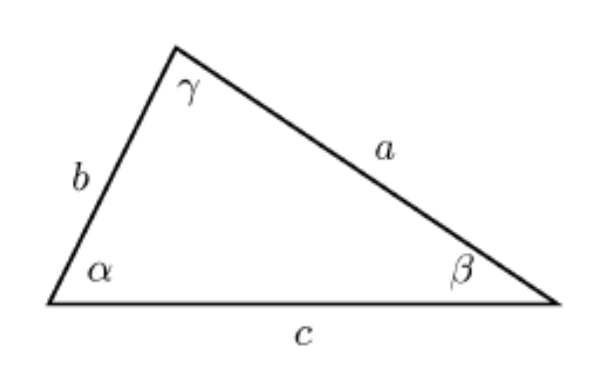
\includegraphics[width=0.5\textwidth]{fig2.1.png}
\end{center}

Fig. 1  Toate funcțiile trigonometrice sunt convexe (sau concave) dacă
argumentele lor sunt limitate la un domeniu adecvat și, în consecință,
există multe consecințe geometrice interesante ale inegalității lui Jensen.


Acum, dacă facem media acestor reprezentări ale ariei, vom obtine că:
\begin{displaymath}
  \frac{1}{3}\left ( ab + ac + bc \right )= \left ( 2A \right )\frac{1}{3}\left \{ \frac{1}{sin \alpha } + \frac{1}{sin \beta } + \frac{1}{sin \gamma }\right \}, \label{eq:2.1} \tag{2.1}
\end{displaymath}
și aceasta este o formulă care ne conduce la a studia convexitatea funcției \(\frac{1}{sin x}\). Reprezentarea grafică a acesteia, \(x \mapsto \frac{1}{sin x}\), pentru \(x\in \left ( 0, \infty  \right )\) cu siguranță este convexă, iar presupunerea noastră poate fi confirmată prin calcularea derivatei a doua,
\begin{displaymath}
  {\left ( \frac{1}{sin x} \right )}''= \frac{1}{sin x} + 2\frac{cos^{2}x}{sin ^{3}x}> 0~~ \text{pentru orice}~~ x\in \left ( 0, \pi  \right )  \label{eq:2.2} \tag{2.2}
\end{displaymath}

	Prin urmare, din moment ce avem \[\frac{\left ( \alpha + \beta  + \gamma  \right )}{3}= \frac{\pi }{3},\] rezultă din inegalitatea lui Jensen că
\begin{displaymath}
  \frac{1}{3}\left \{ \frac{1}{sin \alpha }  + \frac{1}{sin \beta } + \frac{1}{sin \gamma }\right \}\geq \frac{1}{sin \frac{\pi }{3}} =  \frac{2}{\sqrt{3}},
\end{displaymath}
deci, folosind inegalitatea \ref{eq:2.1}, obținem estimarea cerută
\begin{displaymath}
 \max \left ( ab, ac, bc \right )\geq \frac{1}{3}\left ( ab + ac + bc \right )\geq \frac{4}{\sqrt{3}}A. \label{eq:2.3} \tag{2.3}
\end{displaymath}

\end{proof}
\begin{remark}
Această problemă este strâns legată de o inegalitate binecunoscută a lui Weitzenböck care afirmă că în orice triunghi avem
\begin{displaymath}
  a^{2} + b^{2} + c^{2} \geq \frac{4}{\sqrt{3}}A. \label{eq:2.4} \tag{2.4}
\end{displaymath}

De fapt, pentru a trece de la inegalitatea \ref{eq:2.3} la inegalitatea lui Weitzenböck trebuie doar să ne amintim că
\begin{displaymath}
  ab + ac + bc \leq a^{2} + b^{2} + c^{2},
\end{displaymath}
care este o inegalitate bine cunoscută pe care o putem obține în două moduri  - folosind inegalitatea lui Cauchy sau folosind inegalitatea MA-MG

	Inegalitatea lui Weitzenböck se dovedește a avea multe demonstrații instructive - Engel (1998) a dat unsprezece!
Există câteva metode matematice pe care le-am putea numi generic "improvers"; în linii mari, acestea sunt metode care pot fi utilizate într-un mod algoritmic pentru a generaliza o identitate, sau pentru a îmbunătăți un rezultat dat.
\end{remark}
Următoarea problemă oferă un exemplu de alt fel. Aceasta sugerează cum am putea imbunatati aproape orice rezultat care a fost obtinut folosind inegalitatea lui Jensen

\begin{problem}
(Formula defectului a lui Hölder)

Dacă \(f : \left [ a,b  \right ] \to \mathbb{R}\) este derivabilă de doua ori și
\begin{displaymath}
  0 \leq m \leq  f''\left ( x \right ) \leq  M,~ pentru orice ~x\in \left [ a,b \right ], \label{eq:2.5} \tag{2.5}
\end{displaymath}
atunci pentru orice  \(a\leq x_{1}\leq x_{2}\leq ....\leq x_{n} \leq b \) și orice numere reale pozitive \(p_{k}, k= 1,2,.....,n \) cu \(p_{1} + p_{2} + \cdots+ p_{n} = 1\),  există  \(\mu \in \left [ m, M \right ]\) pentru care are loc egalitatea
\begin{displaymath}
  \sum_{k = 1}^{n}p_{k}f\left ( x_{k} \right ) - f\left ( \sum_{k = 1}^{n} p_{k}x_{k}\right ) = \frac{1}{4}\mu \sum_{j = 1}^{n}\sum_{k = 1}^{n}p_{j}p_{k}\left ( x_{j} - x_{k} \right )^{2}. \label{eq:2.6} \tag{2.6}
\end{displaymath}
\end{problem}
\begin{remark}
Acest rezultat provine din aceeași lucrare faimoasă din 1885 a lui Otto Ludwig Hölder (1859 - 1937) în care se găseşte demonstratia inegalităţii care are a ajuns să fie cunoscută  ca ”inegalitatea lui Hölder”. Formula defectului \ref{eq:2.6} este mult mai puțin cunoscută, dar este totuși valoroasă. Aceasta oferă o măsură perfect naturală a diferenței dintre cele două părți ale inegalității lui Jensen și ne spune cum să învingem versiunea  inegalității lui Jensen ori de câte ori putem verifica ipoteza suplimentară \ref{eq:2.5}.
În mod similar, dacă M este mic, să spunem \(0 \leq M \leq \epsilon\), atunci inegalitatea \ref{eq:2.5} ne spune că f se comportă mai degrabă ca o funcție afină, \(f\left ( x \right ) = \alpha  + \beta x\). Pentru o funcție afină, partea stângă a egalitatii \ref{eq:2.6} este identic egală cu zero, dar în general, relația \ref{eq:2.6} afirmă ceva mai subtil. Mai precis, ne spune că partea stângă este un mic multiplu al unei expresii  în care valorile \(x_{j}, j = 1,2,\cdots ,n \) sunt răspandite pe întreg intervalul \(\left [ a, b \right ]. \)
\end{remark}
\begin{proof}
Această problemă ne duce în mod firesc la următoarea întrebare: Cum putem folosi faptul că \(0\leq m\leq {f}''\left ( x \right )\leq M \)?

Odata ce ne-am pus această întrebare, s-ar putea să nu fie nevoie de mult pentru a observa că cele două funcții
\begin{displaymath}
  g\left ( x \right ) = \frac{1}{2}Mx^{2} - f\left ( x \right )~~ și~~
h\left ( x \right ) = f\left ( x \right ) - \frac{1}{2}mx^{2}
\end{displaymath}
sunt doua funcții convexe.
Această observație ne îndeamnă să ne întrebăm ce spune inegalitatea lui Jensen despre aceste funcții.\\
Pentru \(g\left ( x \right )\), inegalitatea lui Jensen ne dă mărginirea
\begin{displaymath}
  \frac{1}{2}M\bar{x}^{2} - f\left ( \bar{x} \right )\leq \sum_{k = 1}^{n}p_{k}\left \{ \frac{1}{2}Mx_{k}^{2} - f\left ( x_{k} \right )\right \}
\end{displaymath}
unde am notat \(\bar{x} = p_{1}x_{1}+ p_{2}x_{2}+ \cdots + p_{n}x_{n}\) și această inegalitate este ușor de rearanjat  pentru a obține
\begin{displaymath}
  \left \{ \sum_{k = 1}^{n} p_{k}f\left ( x_{k} \right )\right \} - f\left (\bar{x}  \right )\leq \frac{1}{2}M\left \{ \left ( \sum_{k=1}^{n} p_{k}x_{k}^{2}\right ) - \bar{x}^{2} \right \} = \frac{1}{2}M\sum_{k = 1}^{n}p_{k}\left ( x_{k} - \bar{x} \right )^{2}.
\end{displaymath}

Un calcul analog pentru  \(h\left ( x \right )\) ne oferă o limită inferioară
\begin{displaymath}
  \left \{ \sum_{k = 1}^{n} p_{k}f\left ( x_{k} \right )\right \} - f\left (\bar{x}  \right )\geq \frac{1}{2}m\sum_{k = 1}^{n}p_{k}\left ( x_{k} - \bar{x} \right )^{2}
\end{displaymath}
și aceste limite superioară și inferioară aproape completează demonstrația egalității  \ref{eq:2.5}. Singurul lucru care lipsește este identitatea
\begin{displaymath}
  \sum_{k = 1}^{n}p_{k}\left ( x_{k} - \bar{x} \right )^{2} = \frac{1}{2}\sum_{j = 1}^{n}\sum_{k = 1}^{n} p _{j}p_{k}\left ( x_{j} - x_{k} \right )^{2}
\end{displaymath}
care se poate verifica usor prin calcul direct folosind definiția lui \(\bar{x}\).
\end{proof}
Comvexitatea și inegalitatea lui Jensen oferă soluții simple pentru multe probleme.
	Următoarea problemă vine din celebra secțiune cu probleme a ”American Mathematical Monthly” si oferă un exemplu clasic al acestei afirmații.
	La început problema pare destul de ușoară, dar, curând, întampinăm dificultăți.

\begin{problem}(AMM 2002, Proposed by M. Mazur)\\
Arătați că dacă a,b și c, sunt numere reale pozitive care verifică \(abc \geq 2^{9}\), atunci
\begin{displaymath}
  \frac{1}{\sqrt{1 + \left ( abc \right )^{\frac{1}{3}}}}\leq \frac{1}{3}\left \{ \frac{1}{\sqrt{1 + a}} + \frac{1}{\sqrt{1 + b}} + \frac{1}{\sqrt{1 + c}}\right \}    	
  \label{eq:2.7} \tag{2.7}
\end{displaymath}
\end{problem}
\begin{proof}
Media din partea dreaptă sugerează că inegalitatea lui Jensen s-ar putea dovedi utilă, în timp ce media geometrică din partea stângă sugerează că funcția exponențială va avea un rol.

Dacă ne uităm mai atent, putem observa că
\begin{displaymath}
  f\left ( x \right ) = \frac{1}{\sqrt{1+ e^{x}}}
\end{displaymath}
ne poate ajuta la folosirea inegalității lui Jensen. De fapt, odată ce am scris această funcție, se poate verifica aproape fără calcul că inegalitatea propusă \ref{eq:2.7} este echivalentă cu
\begin{displaymath}
  f\left ( \frac{x + y + z}{3} \right )\leq \frac{1}{3}\left \{ f\left ( x \right ) + f\left ( y \right ) + f\left ( z \right ) \right \}    \label{eq:2.8} \tag{2.8}
\end{displaymath}
pentru orice $x, y, z$ astfel încât \(\exp\left ( x + y + z \right )\geq 2^{9}.\)

Pentru a vedea dacă putem aplica inegalitatea lui Jensen, trebuie să evaluăm convexitatea lui f. Într-adevar, avem

\begin{center}
	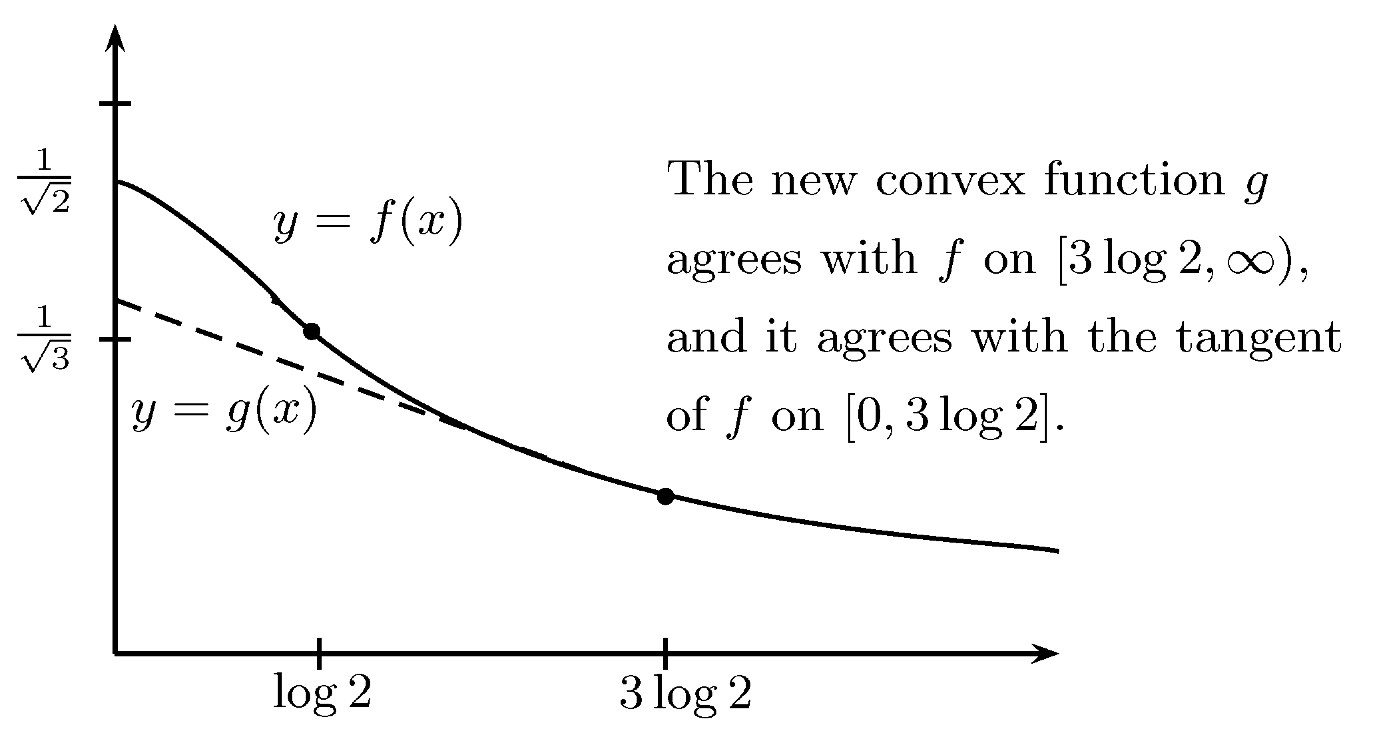
\includegraphics[width=1.0\textwidth]{fig_pb3.png}
\end{center}

\begin{displaymath}
  {f}'\left ( x \right ) = -\frac{e^{x}}{2 \left ( 1 + e^{x} \right )^{\frac{3}{2}}}
\end{displaymath}
si
\begin{displaymath}
  {f}''\left ( x \right ) = -\frac{1}{2}\left (  1 + e^{x} \right )^{-\frac{3}{2}}e^{x} + \frac{3}{4}\left ( 1 + e^{x} \right )^{-\frac{5}{2}}e^{2x}
\end{displaymath}

Cea de a doua egalitate ne arată ca\({f}''\left ( x \right ) \geq 0\) dacă și numai dacă avem \(e^{x}\geq 2\), atfel încât cu ajutorul inegalității lui Jensen  constatăm că inegalitatea inițiala \ref{eq:2.8}  este adevarată cu condiția ca fiecare dintre termenii a, b si c să fie mai mari sau egali cu2.

Dificultatea cu care ne confruntăm aici este că ipoteza problemei  ne spune doar  că produsul \(abc\) este mai mare sau egal cu \(2^{9}\); nu ni se da nicio  limită pentru termenii  individuali, cu excepția faptului că \( a > 0, b > 0 \) si \(c > 0\) . Astfel, inegalitatea lui Jensen nu poate completa demonstrația de la sine și noi trebuie să cautăm alte informații.

Există multe idei pe care le-am putea încerca, dar inainte de a merge prea departe,  ar trebui să luăm în considerare graficul lui \(f\left ( x \right )\). Ceea ce  găsim  din graficul  reprezentat în Figura 3 este că \(f\left ( x \right ) \) arată convexă pe interval \(\left [ 0, 10 \right ]  \), în ciuda faptului că calculul care arată că \(f\left ( x \right ) \) este concavă pe \(\left [ 0, \log _{} 2\right ] \) și convexă pe \(\left [ \log _{} 2 , \infty \right ) \). Astfel, graficul nostru oferă o noua speranță; poate că o mica modificare a lui \(f\) ar putea conduce la convexitatea de care noi avem nevoie pentru a rezolva problema.

Când ne gandim la modul în care am sperat să folosim \(f\) cu inegalitatea lui Jensen, în curând ne dăm seama că ne putem ușura puțin sarcina. Să presupunem, de exemplu, că putem gasi o funcție convexă \(g : \left [ 0 , \infty  \right ) \to \mathbb{R}\) astfel încât sa avem  conditiile:
\begin{displaymath}
  g\left ( x \right ) \leq  f\left ( x  \right ),~~ pentru~~ orice~~ x \in  \left [ 0 , \infty  \right )    \label{eq:2.9} \tag{2.9}
\end{displaymath}
și condiția complementară
\begin{displaymath}
  g \left ( x \right ) = f \left ( x \right ), ~~pentru~~ orice~~  x\geq 3 \log 2. \label{eq:2.10} \tag{2.10}
\end{displaymath}

Pentru o astfel de funcție, inegalitatea lui Jensen ne spune  că dacă x,y și z verifică \[exp \left ( x + y + z \right )\geq  2^{9} \] avem inegalitațile
\begin{displaymath}
\begin{split}
  f\left ( \frac{x + y + z}{3} \right ) &= g\left ( \frac{x + y + z}{3} \right )\\
   &\leq  \frac{1}{3}\left \{ g\left ( x \right ) + g\left ( y \right ) + g\left ( z \right ) \right \} \leq  \frac{1}{3}\left \{ f\left ( x \right ) + f\left ( y \right ) + f\left ( z \right ) \right \}.
  \end{split}
\end{displaymath}

Primul și ultimul termen al acestei inegalități conduc la inegalitatea \ref{eq:2.8}, deci soluția problemei ar fi completă, cu excepția unui mic detaliu — mai trebuie să arătăm că există o functie  g convexă pe \( \left [ 0 , \infty  \right ) \) astfel încat  \(g\left ( x \right ) \leq  f\left ( x \right )\) pentru orice  \(x \in \left [ 0 , 3\log 2 \right ]\) și \( f\left ( x \right ) = g\left ( x \right )\) pentru orice \( x \geq 3\log 2\).

O modalitate de a construi o funcție convexă \(g\) cu proprietățile  descrise mai sus este să luăm  \(g\left ( x \right ) = f\left ( x \right )\) pentru \(x \geq  3\log2\) și să definim \(g\left ( x \right )\) pe \(\left [ 0 , 3\log 2 \right ]\) prin extrapolare liniară. Astfel, pentru \(x\in \left [ 0 , 3\log 2 \right ]\), luăm
\begin{displaymath}
  g\left ( x \right ) - f\left ( 3\log 2 \right ) + \left ( x - 3\log 2 \right ){f}'\left ( 3\log2 \right ) = \frac{1}{3} + \left ( 3\log2 - x  \right )\left ( \frac{4}{27} \right )
\end{displaymath}

Trei observatii simple sunt acum suficiente pentru a demonstra că \(g\left ( x \right )\leq f\left ( x \right )\), pentru orice \(x\geq 0\). Pentru inceput, pentru \(x\geq 3\log 2\), avem \(g\left ( x \right ) = f\left ( x \right )\) din definiție.

Cea de a doua observație, pentru \(\log 2 \leq  x \leq  3\log 2\) avem  \(g( x )\leq f\left ( x \right ) \) pentru ca aici  \(g\left ( x \right )\) are valoarea unei drepte tangente la \((f\left ( x \right )\) și din convexitatea lui f pe \(\log 2 \leq  3 \leq 3\log 2\) dreapta tangentă este sub f.

Cea de a treia observație, în regiunea critică \(0\leq  x \leq \log2\), avem \(g\left ( x \right ) \leq  f\left ( x \right )\) deoarece,
\begin{enumerate}
  \item f este concavă,
  \item g este liniară,
  \item f este mai mare decât \(g\) la capetele intervalului \(\left [ 0 , \log 2 \right ]\).
\end{enumerate}
Mai precis, avem
\begin{displaymath}
  g\left ( 0 \right ) = 0.641\cdots \leq f\left ( 0 \right ) = \frac{1}{\sqrt{2}} = 0.707\cdots,
\end{displaymath}
în timp ce în cel de-al doilea punct avem
\begin{displaymath}
  g\left ( \log 2 \right ) = 0.538\cdots  \leq f\left ( \log2 \right ) = \frac{1}{\sqrt{3}} = 0.577\cdots.
\end{displaymath}
Astfel, funcția convexă \(g\) este într-adevar un minorant al funcției \(f\) care se află în concordanță cu \(f\) pe \(\left [ 3\log 2 , \infty  \right )\), așadar rezolvarea problemei este completă.
\end{proof}
\begin{problem} (O inegalitate renascentistă)\\
   Matematicianul renascentist Pietro Mengoli (1625 – 1686) a avut nevoie doar de algebra elementară pentru a demonstra inegalitatea
 \begin{displaymath}
   \frac{1}{x - 1} + \frac{1}{x} + \frac{1}{x + 1} > \frac{3}{x} , \text{pentru orice } x > 1, \label{eq:2.11} \tag{2.11}
 \end{displaymath}
totuși a obținut o revendicare asupra numuririi intelectuale atunci când a folosit asta pentru a oferi una dintre cele mai timpurii dovezi ale divergenței seriilor armonice,
\begin{displaymath}
  H_{n} = 1 + \frac{1}{2} + \frac{1}{3} + \cdots + \frac{1}{n} \Rightarrow \lim_{n \to \infty } H_{n} = \infty \label{eq:2.12} \tag{2.12}
\end{displaymath}

Redescoperiți demonstrația algebrică a inegalității lu Mengoli (2.4.1) și verificați faptul că rezultă și din inegalitatea lui Jensen. Mai departe, arătați, cum a facut Mengoli, faptul că inegalitatea \ref{eq:2.11} implică divergența lui \(H_{n}\) .
\end{problem}
\begin{proof}
Simplificând \(\frac{1}{x}\) din ambele parți și adunând fracțiile se vede că inegalitatea lui Mengoli este echivalentă cu inegalitatea  trivială \(x^{2} >  x^{2} – 1\). \\
Pentru o demonstrație folosind inegalitatea lui Jensen, observăm că \(x \mapsto \frac{1}{x}\) este stict convexă. Aplicăm inegalitatea lui Jensen pentru $x_1=x-1,$ $x_2=x,$ $x_3=x-1,$ si $\lambda_i=1/3,~i=1, 2, 3:$
\[
f\biggl(\frac{1}{3}(x-1+x+x+1)\biggr)=f(x)<\frac{1}{3}f(x+1)+\frac{1}{3}f(x)+\frac{1}{3}f(x-1)\Leftrightarrow
\]
\[
\frac{1}{x}<\frac{1}{3}\frac{1}{x+1}+\frac{1}{3}\frac{1}{x}+\frac{1}{3}\frac{1}{x-1}
\]
care inmulțită cu trei este inegalitatea lui Mengoli.\\
În final, pentru o versiune modernă a demonstrației lui Mengoli că \(H_{n}\) diverge, presupunem prin absurd că \(H_{\infty }< \infty\) și scriem \(H_{\infty }\) că
\begin{displaymath}
  1 + \left ( \frac{1}{2} + \frac{1}{3} + \frac{1}{4} \right ) + \left ( \frac{1}{5} + \frac{1}{6} + \frac{1}{7} \right ) + \left ( \frac{1}{8} + \frac{1}{9} +\frac{1}{10} \right )+\cdots.
\end{displaymath}

Acum, prin aplicarea inegalității lui Mengoli în cadrul grupurilor formate găsim că
\[
H_{\infty }>1 + \frac{3}{3} + \frac{3}{6} + \frac{3}{9} + ..= 1 + H_{\infty }
\]
care ne conduce la contradicția \(H_{\infty } > 1 + H_{\infty }\).
\end{proof}
\begin{remark}
Potrivit lui Havil, Mengoli a fost cel care a propus pentru prima data problema determinării valorii sumei \[1 + \frac{1}{2^{2}} + \frac{1}{3^{2}} + \cdots.\]
Problema a rezistat eforturilor celor mai buni matematicieni ai Europei până în anul 1731 când L. Euler a determinat valoarea ca fiind \(\frac{\pi^{2}}{6}\).
\end{remark}

\begin{problem}
Arătați că dacă \(x , y , z > 0\) si \(x+ y + z = 1\), atunci
\begin{displaymath}
  64 < \left ( 1 + \frac{1}{x} \right )\left ( 1 + \frac{1}{y} \right )\left ( 1 + \frac{1}{z} \right ).
\end{displaymath}
\end{problem}
\begin{proof}
Inegalitatea rezultă prin aplicarea inegalității lui Jensen funcției
\begin{displaymath}
  f\left ( t \right ) = \ln \left ( 1+\frac{1}{t} \right ) = \ln \left ( 1 + t \right ) - \ln \left ( t \right ),~t>0
\end{displaymath}
care este strict convexă deoarece
\begin{displaymath}
  {f}''\left ( t \right ) = -\frac{1}{\left ( 1 + t \right )^{2}} + \frac{1}{t^{2}} > 0,  \text{pentru orice } t > 0.
\end{displaymath}

Într-adevar, pentru  $x_1=x,$ $x_2=y,$ $x_3=z,$ si $\lambda_i=1/3,~i=1, 2, 3:$
\[
f\biggl(\frac{1}{3}(x+y+z)\biggr)=f\biggl(\frac{1}{3}\biggr)<\frac{1}{3}f(x)+\frac{1}{3}f(y)+\frac{1}{3}f(z)\Leftrightarrow
\]
\[
\ln (4)<\frac{1}{3}\ln\biggl(1+\frac{1}{x})\biggr) +\frac{1}{3}\ln\biggl(1+\frac{1}{y}\biggr)+\frac{1}{3}\ln\biggl(1+\frac{1}{z}\biggr)\Leftrightarrow
\]
\[
3\ln (4)< \ln\biggl((1+\frac{1}{x})(1+\frac{1}{y})(1+\frac{1}{z})\biggr)
\]
și aplicând exponențiala obținem inegalitatea dorită.
\end{proof}


\begin{problem} (Inegalitatea ariei n-poligonului)

Figura 4 sugerează că  dintre toate poligoanele convexe cu n laturi care pot fi înscrise într-un cerc, numai n-gonul regulat are aria maximă. Poate inegalitatea lui Jensen să fie folosită pentru a confirma această afirmație?

\begin{center}
	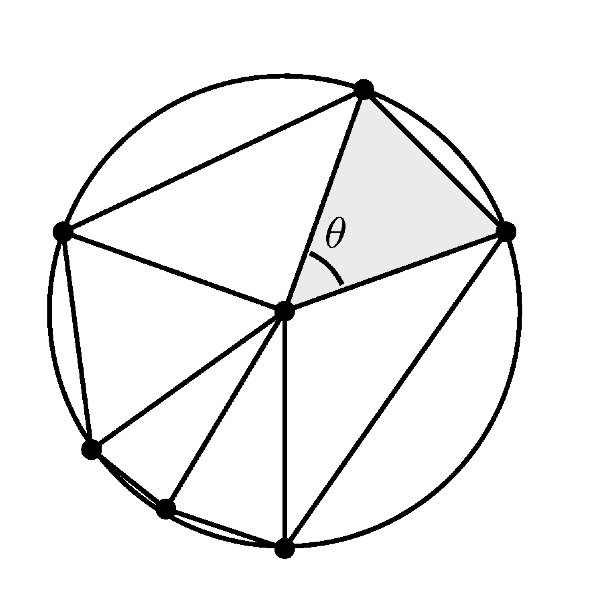
\includegraphics[width=0.5\textwidth]{fig_pb6.png}
	\\ Figura 4
\end{center}
\end{problem}
\begin{proof}
Din figura geometrică precizată, dacă presupunem fără a restrange generalitatea că raza cercului este 1, aria A a unui poligon înscris cu n laturi poate fi scrisă ca
\begin{displaymath}
  A = \frac{1}{2}\sum_{k = 1}^{n} \sin \theta _{k} ~~unde ~~0< \theta _{k} ~~si~~ \sum_{k = 1}^n{\theta _{k}} = 2\pi.
\end{displaymath}
	Cum funcția  \(\sin \left ( \cdot  \right )\) este strict concavă pe \(\left [ 0 , \pi  \right ]\), folosind inegalitatea lui Jensen avem
\begin{displaymath}
  A = \frac{1}{2}\sum_{k = 1}^{n} \sin \theta _{k}  \leq \frac{1}{2}n\sin\left ( \frac{1}{n}\sum_{k = 1}^{n}\theta _{k} \right ) = \frac{1}{2}n\sin \left ( \frac{2\pi }{n} \right ) = {A}'
\end{displaymath}
și avem egalitate dacă și numai dacă \(\theta _{k} = \frac{2\pi }{n}\) pentru orice \(1\leq k\leq n\). Cum \({A}'\) este aria unui n-poligon regulat înscris, optimalitatea presupusă este confirmată.
\end{proof}

\begin{problem} (Inegalitățile investiționale)

Dacă \(0< r_{k} < \infty\). Dacă investiția noastră de un dolar în anul \(k\) crește la \(1 +  r_{k}\) dolari la sfârșitul anului, numim \(r_{k}\) dobânda investităției în anul \(k\). Demonstrați că valoarea
\begin{displaymath}
  V = \left ( 1 + r_{1} \right )\left ( 1 + r_{2} \right )\cdots \left ( 1 + r_{n} \right )
\end{displaymath}
a investiției noastre după n ani verifică inegalitățile
\begin{displaymath}
  \left ( 1 + r_{G} \right )^{n} \leq \prod_{k = 1}^{n} \left ( 1 + r_{k} \right )\leq \left ( 1 + r_{A} \right )^{n}, \label{eq:2.13} \tag{2.13}
\end{displaymath}
unde
\begin{displaymath}
  r_{G} = \left ( r_{1}r_{2} \cdots r_{n}\right )^{\frac{1}{n}}~~ si~~ r_{A} = \frac{\left ( r_{1} + r_{2} +  \cdots+ r_{n}\right )}{n}.
\end{displaymath}
De asemenea explicați de ce aceaste inegalități  pot fi vazute ca un rafinament al inegalității MA-MG.
\end{problem}
\begin{proof}
Evident, inegalitatea din dreapta rezultă imediat dacă aplicăm inegalitatea MA-MG pentru
\begin{displaymath}
  a_{k} = 1 + r_{k},~ k =1,2,\cdots, n.
\end{displaymath}
Pentru inegalitatea din partea stângă aplicăm inegalitatea lui Jensen aplicată funcției convexe
\[x \mapsto \ln\left ( 1 + e^{x} \right ).\]
Evident, dacă notăm cu $f$ această funcție, observăm că
\[
f''(x)=\frac{e^x}{(1+e^x)^2}>0,
\]
deci f este chiar strict convexă. Dacă aplicăm inegalitatea lui Jensen acestei funcții pentru
\[
x_1=\ln r_1,\cdots, x_1=\ln r_1,~~\lambda_1=\frac{1}{n},\cdots, \lambda_n=\frac{1}{n},
\]
deducem și inegalitatea din stânga.\\
La final, dacă extragem rădăcina de ordinul n și scădem 1, în toți termenii, vom vedea că inegalitatea \ref{eq:2.13} rafinează limita MA-MG,  \(r_{G} \leq r_{A}\) prin intercalarea termenului \(V^{\frac{1}{n}} – 1\) între cele două.
\end{proof}

\begin{problem} (Supraaditivitatea mediei geometrice)
	
Dacă \(a_{j}\geq 0 \) si \(b_{j}\geq 0, j = 1 , 2, \cdots, n,\) atunci:
\begin{displaymath}
  \left ( a_{1}a_{2}\cdots a_{n} \right )^{\frac{1}{n}} + \left ( b_{1}b_{2}\cdots b_{n} \right )^{\frac{1}{n}} \leq  \left \{ \left ( a_{1} + b_{1}\right ) \left ( a_{2} + b_{2} \right )\cdots \left ( a_{n} + b_{n} \right )\right \}^{\frac{1}{n}}.
\end{displaymath}
\end{problem}
	\begin{proof}
	Pentru a construi o demonstrație cu ajutorul inegalității lui Jensen, mai întâi împărțim la
\(\left ( a_{1}a_{2}\cdots a_{n} \right )^{\frac{1}{n}}\) și notăm \(c_{k}=\frac{b_{k}}{a_{k}},~k=1,\cdots, n\) deci inegalitatea de la care am pornit devine
\begin{displaymath}
  1 + \left ( c_{1}c_{2} \cdots c_{k}\right )^{\frac{1}{n}}\leq \left \{ \left ( 1 + c_{1} \right )\left ( 1 + c_{2} \right )\cdots \left ( 1 + c_{n} \right ) \right \}^{\frac{1}{n}}.
\end{displaymath}

Acum, dacă scriem \(c_{j}\) ca \(exp\left (d _{j} \right )\), vom vedea că obținem forma echivalentă
\begin{displaymath}
  \ln\left ( 1 + exp\left ( \bar{d} \right ) \right ) \leq \frac{1}{n}\sum_{j = 1}^{n}\ln\left ( 1 + exp\left ( d_{j} \right ) \right ),
\end{displaymath}
unde
\begin{displaymath}
  \bar{d} = \frac{\left ( d_{1} + d_{2}  + \cdots + d_{n}\right )}{n}.
\end{displaymath}
Obsevăm acum că ultima inegalitate este pur și simplu inegalitatea lui Jensen pentru funcția convexă \(x \mapsto \log \left ( 1 + e^{x} \right )\), astfel, rezolvarea este completă.
\end{proof}
\begin{remark}
O caracteristică a acestei soluții care merită remarcată este aceea că progresul în rezolvarea problemei a venit rapid după ce împarțirea a redus numărul de variabile de la \(2n\) la \(n\). Acest fenomen este de fapt destul de comun și astfel de reduceri merită aproape întotdeauna încercate.
\end{remark}

\begin{problem} (Technica lui Cauchy și Inegalitatea lui Jensen)

În 1906, J. L. W. V. Jensen a scris un articol care a fost inspirat de demonstrația dată de Cauchy pentru inegalitatea MA-MG și, într-un efort de a ajunge la miezul argumentului lui Cauchy, Jensen a introdus clasa de funcții care satisfac inegalitatea
\begin{displaymath}
  f\left ( \frac{x + y}{2} \right ) \leq \frac{f\left ( x \right ) + f\left ( y \right )}{2} \text{pentru orice } x,y \in \left [ a, b \right ]. \label{eq:2.14} \tag{2.14}
\end{displaymath}

Astfel de funcții sunt acum numite funcții J-convexe și, după cum observăm mai jos în problema care urmează, ele sunt doar puțin mai generale decât funcțiie convexe definite de condiția
\begin{displaymath}
  f\left ( px + \left ( 1 - p \right )y \right )\leq pf\left ( x \right ) + \left ( 1-p \right )f\left ( y \right ).
\end{displaymath}

Să se arate că orice funcție  J-convexă verificaă inegalitatea
\begin{displaymath}
  f\left ( \frac{1}{n} \sum_{k = 1}^{n}x_{k}\right )\leq \frac{1}{n}\sum_{k = 1}^{n}f\left ( x_{k} \right )
\end{displaymath}
pentru orice
\begin{displaymath}
  \left \{ x_{k}: 1\leq k \leq n \right \} \subset \left [ a, b \right ]. \label{eq:2.15} \tag{2.15}
\end{displaymath}
\end{problem}
\begin{proof}
Vom aplica thenica pe care Cauchy a folosit-o pentru a demonstra inegalitatea mediilor. Astfel, pentru început presupunem că \(n = 2^{k}, k=1,2,….,\) și demonstrăm \ref{eq:2.15} în acest caz.

Într-adevar, dacă luăm în \ref{eq:2.14} $x=(x_1+x_2)/2$ si $y=(x_3+x_4)/2$ vom obține că
\begin{equation*}
  f\left ( \frac{x_1 + x_2+x_3+x_4}{4} \right ) \leq \frac{f\left ( \frac{x_1 + x_2}{2} \right) + f\left(\frac{x_3 + x_4}{2} \right )}{2} \leq
\end{equation*}
\begin{equation*}
   \frac{f\left (x_1) + f\left (x_2 \right )+f\left (x_3 \right )+f\left (x_4 \right ) \right)}{4} \text{pentru orice } x_1, \cdots, x_4 \in \left [ a, b \right ]\leq
\end{equation*}
Repetând procedeul obținem \ref{eq:2.15} pentru orice $n=2^k,~k\geq 1.$\\
 Pentru a demonstra acum în cazul în care $n$ nu e de forma anterioară, alegem  \(k\) astfel încat \(n< 2^{k}\) și aplicăm rezultatul pentru \(2^{k}\) șirului de valori \(y_{j} , 1\leq j\leq 2^{k}\) luând \(y_{j} = x_{j}\) pentru \(1\leq j\leq n \) si \(y_{j} = \frac{\left ( x_{1} + x_{2} + ....+ x_{n} \right )}{n}=\overline{x}\) pentru \(n< j\leq 2^{k}\), astfel vom avea
 \[
   f\left ( \frac{x_1 + \cdots+x_n}{2^k}+\frac{x}{2^k}+\cdots+\frac{x}{2^k} \right )=f\left( \frac{n \overline{x}}{2^k}+\frac{(2^k-n) \overline{x}}{2^k}\right)=f(\overline{x}) \leq
 \]
 \[
\frac{ f(x_1)}{2^k}+\cdots+\frac{ f(x_n)}{2^k}+\frac{(2^k-n)}{2^k}f(\overline{x})=\frac{ f(x_1)}{2^k}+\cdots+\frac{ f(x_n)}{2^k}+ (1-\frac{n}{2^k})f(\overline{x})
 \]
 care va implica
 \[
 f(\overline{x})=  f\left ( \frac{x_1 + \cdots+x_n}{n} \right )\leq f\left ( \frac{x_1}{n} \right )+\cdots+f\left ( \frac{x_n}{n} \right ),
 \]
 adică inegalitatea \ref{eq:2.15}.
\end{proof}

\begin{problem}  (Convexitatea si J-Convexitatea)

Demonstrați că dacă \(f : \left [ a,b \right ]\rightarrow \mathbb{R} \) este continuă și J-convexă, atunci \(f\) trebuie să fie convexă, adică pentru orice $x, y\in [a,b],~ p\in [0,1]$
\begin{displaymath}
  f\left ( px + \left ( 1 - p \right )y \right )\leq pf\left ( x \right ) + \left ( 1-p \right )f\left ( y \right.
\end{displaymath}
\end{problem}
\begin{remark}
Ca o curiozitate, ar trebui să punctăm faptul că există funcții J-convexe care nu sunt convexe. Cu toate acestea, astfel de funcții sunt discontinue și foarte rar utilizate.
\end{remark}
\begin{proof}
După cum am observat în soluția anterioară, avem că pentru orice \(k = 1,2,\cdots\) are loc inegalitatea
\begin{displaymath}
  f\left ( \frac{1}{2^{k}} \sum_{j = 1}^{2^{k}}x_{j}\right ) \leq  \frac{1}{2^{k}}\sum_{j = 1}^{2^{k}}f\left ( x_{j}\right ),
\end{displaymath}
deci luând \(x_{j} = x\) pentru \(1\leq j\leq m\) si \(x_{j} = y\) pentru \(m< j\leq 2^{k}\) avem de asemenea
\begin{displaymath}
  f\left ( \left ( \frac{m}{2^{k}} \right )x + \left ( 1 - \frac{m}{2^{k}} \right )y \right )\leq \left ( \frac{m}{2^{k}} \right )f\left ( x \right ) + \left ( 1 - \frac{m}{2^{k}} \right )f\left ( y \right ).
\end{displaymath}
Dacă alegem acum \(m_{t}\) si \(k_{t}\) astfel încât \(\frac{m_{t}}{2^{k_{t}}} \rightarrow p\) pentru \(t \rightarrow \infty\), atunci continuitatea lui f și inegalitatea precedentă vor implica
\begin{displaymath}
  f\left ( px + \left ( 1 - p \right )y \right ) \leq  pf\left ( x \right ) + \left ( 1 - p \right )f\left ( y \right ).
\end{displaymath}
\end{proof}

\begin{problem}
	Arătați că pentru orice \(0\leq x , y , z \leq 1\), una are limita
\begin{displaymath}
  L\left ( x , y , z \right ) = \frac{x^{2}}{1 + y} + \frac{y^{2}}{1 + z} + \frac{z^{2}}{1 + x+ y} + x^{2} \left ( y^{2} - 1 \right )\left ( z^{2} - 1 \right ) \leq 2.
\end{displaymath}
\end{problem}
\begin{proof}
Funcția \(L\left ( x,y,\ \right )\) este convexă în fiecare din cele trei variabile ale sale separat și prin argumentul detaliat mai jos, acest lucru implică faptul că L trebuie să atingă punctul maxim  în unul dintre vârfurile cubului.

După opt evaluari ușoare constatăm că \(L \left ( 1,0,0 \right ) = 2\) și că în niciun alt colț al cubului $[0, 1]^3$ L nu are o valoare mai mare, deci soluția va fi completă. Este de asemenea ușor să arătaăm că dacă o funcție definită pe cub este convexă în fiecare variabilă separat, atunci funcția trebuie să atingă maximul în unul dintre varfuri.

În primul rând se observă ca o funcție convexă pe \(\left [ 0 , 1 \right ]\) trebuie să iși atingă maximul în unul dintre punctele finale ale intervalului, deci, pentru orice valoare fixă dintre y și z, avem inegalitatea
\begin{displaymath}
  L\left ( x,y,z \right )\leq max \left \{ L\left ( 0,y,z \right ), L\left ( 1,y,z \right ) \right \}.
\end{displaymath}

 Similar din convexitatea lui \(y \mapsto L\left ( 0,y,z \right )\) si \(y \mapsto L\left ( 1,y,z \right )\)  rezultă că \(L\left ( 0, y, z \right )\) este marginit superior de  \[\max \{L\left ( 0,0,z \right ), L\left ( 0,1,z \right )\}\] si \( L\left ( 1,y,z \right )\) este marginit superior de \[\max \{\left \{ L\left ( 1,0,z \right ) , L \left ( 1,1,z \right )\right \}\}.\]

 Luând toate aceste marginiri superioare, avem pentru orice valoare a lui z că \(L\left ( x,y,z \right )\) este marginita de
 \[\max\left \{ L\left ( 0,0,z \right ), L\left ( 0,1,z \right ), L\left ( 1,1,z \right ) \right \}.\]

 Convexitatea lui \(z \mapsto L\left ( x,y,z \right )\) aplicată de patru ori ne dă apoi marginirea
 \begin{displaymath}
  L\left ( x,y,z \right ) \leq  \max \left \{ L\left ( e_{1} , e_{2}, e_{3}\right ): e_{k}  = 0 \text{sau } e_{k} = 1 ~\text{pentru }~ k = 1,2,3\right \}
\end{displaymath}
\end{proof}


\begin{problem}
Pentru orice triunghi, teorema cosinusului care ne spune că
\begin{displaymath}
  a^{2} = b^{2}+ c^{2} - abc\cos\alpha.
\end{displaymath}
Araătatți că această teoremă implică formula ariei
\begin{displaymath}
  a^{2} = \left ( b - c^{2} \right ) + 4 A\tan \left ( \frac{\alpha }{2} \right ),
\end{displaymath}
apoi arătați cum implică inegalitatea lui Jensen faptul că în orice triunghi
\begin{displaymath}
  a^{2} + b^{2} + c^{2} \geq  \left ( a - b  \right )^{2} + \left ( b- c  \right )^{2} + \left ( c - a \right )^{2} + 4\sqrt{3}A.
\end{displaymath}
\end{problem}
\begin{proof}
Această inegalitate este cunoscută ca inegalitatea Hadwiger-Finsler , și furnizează una din cele mai frumoase rafinamente ale inegalității Weitzenböck.

Pentru a demonstra prima formulă, observăm că
\begin{displaymath}
  a^{2} = b^{2} + c^{2} - 2ac\cos\alpha  = \left (  b - c \right )^{2} + 2bc\left ( 1 - \cos\alpha  \right )=
\end{displaymath}
\begin{displaymath}
 \left ( b - c \right )^{2} + \frac{4A\left ( 1 - \cos  \right )}{\sin \alpha } = \left ( b - c \right )^{2} + 4A\tan\left ( \frac{\alpha }{2} \right ),
\end{displaymath}
deci, prin simetrie și adunare, vedem că
\(a^{2} + b^{2} + c^{2}\) este egal cu
\begin{displaymath}
  \left ( a - b  \right )^{2} + \left ( b - c \right )^{2} + \left ( c - a  \right )^{2} + 4A\left ( \tan\left ( \frac{\alpha }{2} \right ) + \tan\left ( \frac{\beta }{2} \right ) + \tan \frac{\gamma }{2} \right ).
\end{displaymath}
	Cum \(x \mapsto \tan x\) este convexă pe \(\left [ 0 , \frac{\pi }{2} \right ]\), inegalitatea lui Jensen implică
\begin{displaymath}
  \frac{1}{3}\left \{ \tan \left ( \frac{\alpha }{2} \right ) + \tan \left ( \frac{\beta }{2} \right )  + \tan \left ( \frac{\gamma }{2} \right )\right \} \geq  \tan\left ( \frac{\alpha  + \beta  + \gamma }{6} \right ) = \tan \left ( \frac{\pi }{6} \right)
\end{displaymath}

Și cum\(\tan \left ( \frac{\pi }{6} \right ) = \sqrt{3}\),  am incheiat demonstrația.
\end{proof}

\begin{problem} (Criteriul derivatei secunde și Teorema lui Rolle)
	
Este cunoscut faptul că dacă \({f}'' \geq 0\) pentru orice \(x\in \left [ a,b \right ]\), atunci \(f\) este convexă pe \(\left [ a,b \right ]\). Acest exercițiu schițează cum se poate demonstra acest lucru important prin estimarea diferenței
\begin{displaymath}
  f\left ( px_{1} + qx_{2}\right ) - pf\left ( x_{1} \right ) - qf\left ( x_{2} \right ).
\end{displaymath}
 prin compararea cu un polinom.
 \begin{enumerate}[a)]
\item Luăm \(0< p < 1, q = 1-p\) și notăm \(mu = px_{1} + px_{2}\) unde \(x_{1} < x_{2}\).  Gasiți polinomul pătratic unic \(Q\left ( x \right )\) astfel încât  \(Q\left ( x_{1} \right ) = f\left ( x_{1} \right ), Q\left ( x_{2} \right ) = f\left ( x_{2} \right )\) si \(Q\left ( \mu  \right ) = f\left ( \mu  \right )\).
\item Folosind faptul că \(\Delta \left ( x \right ) =  f\left ( x \right ) - Q\left ( x \right )\) are trei zerouri distincte în \(\left [ a,b \right ]\) pentru a demosntra că există un \(x^{*}\) astfel încât \({\Delta }''\left ( x^{*} \right ) = 0\).
\item În final, explicați cum \({f}''\left ( x \right ) \geq 0\) pentru orice \(x\in \left [ a,b \right ]\) si \({\Delta }''\left ( x^{*} \right ) = 0\) implică faptul că \(f\left ( px_{1} + qx_{2} \right ) - pf\left ( x_{1} \right ) - qf\left ( x_{2} \right ) \geq 0\).
\end{enumerate}
\end{problem}
\begin{proof}
Polinomul \(Q\left ( x \right )\) poate fi scris astfel:
\begin{displaymath}
  \frac{\left ( x - x_{2} \right )\left ( x - \mu  \right )}{\left ( x_{1}  - x_{2}\right )\left ( x_{1} - \mu  \right )} f\left ( x_{1} \right ) + \frac{\left ( x - x_{1} \right )\left ( x - \mu  \right )}{\left ( x_{2}  - x_{1}\right )\left ( x_{2} - \mu  \right )}  f\left ( x_{2} \right ) +  \frac{\left ( x - x_{1} \right )\left ( x - x_{2}  \right )}{\left ( \mu   - x_{1}\right )\left (  \mu - x_{2} \right )}f\left ( \mu \right ).
\end{displaymath}
După ce aplicăm Teorema lui Rolle de doua ori observăm faptul că  \({Q}'\left ( x \right ) - {f}'\left ( x \right )\) are un zero în \(\left ( x_{1} , \mu \right )\) și un alt zero în \(\left ( \mu  , x_{2} \right )\), deci o a treia aplicare a Teoremei lui Rolle ne arată că există un \(x^{*}\) între aceste zerouri pentru care avem \(0 = {Q}''\left ( x \right ) - {f}''\left ( x^{*} \right )\). Prin urmare o să avem \({Q}''\left ( x^{*}  \right ) = {f}''\left ( x^{*} \right )\geq 0\). Dar
\begin{displaymath}
  {Q}''\left ( x^{*}  \right ) = \frac{2f\left ( x_{1} \right )}{\left ( x_{1} - x_{2} \right )\left ( x_{1} - \mu  \right )} +  \frac{2f\left ( x_{2} \right )}{\left ( x_{2} - x_{1} \right )\left ( x_{2} - \mu  \right )} +  \frac{2f\left (\mu  \right )}{\left ( \mu  - x_{1} \right )\left ( \mu  - x_{2} \right )}
\end{displaymath}
Deci, luând
\begin{displaymath}
  p = \frac{\left ( x_{2} - \mu  \right )}{\left ( x_{2} - x_{1}\right )}
\end{displaymath}
și
\begin{displaymath}
  q = \frac{\left ( \mu  - x_{1} \right )}{\left ( x_{2} - x_{1} \right )}
\end{displaymath}
și simplificând, se constată că ultima inegalitate se reduce la definiția convexității lui f.
\end{proof}
\begin{problem} (Transformare pentru obținerea convexității)
Arătați că pentru numere pozitive \(a , b si c\) care verifică \(a + b = c = abc\), avem
\begin{displaymath}
  \frac{1}{\sqrt{1 + a^{2}}} + \frac{1}{\sqrt{1 + b^{2}}} + \frac{1}{\sqrt{1 + c^{2}}} \leq \frac{3}{2}
\end{displaymath}
\end{problem}
\begin{proof}
Această problemă dată la Olimpiada Națională din Koreea în 1998 nu este ușoară, chiar și cu indicația oferită de titlul exercițiului. Cineva, care este norocos, poate stabili o legătură între  ipoteza \(a + b + c = abc\) și binecunoscutul lucru ca într-un triunghi, cu notațiile  ca în figura Fig 1
 avem
 \begin{displaymath}
   \tan\left ( \alpha  \right ) + \tan\left ( \beta   \right ) + \tan\left ( \gamma   \right ) = \tan\left ( \alpha  \right )\tan\left ( \beta   \right )\tan\left ( \gamma   \right ).
 \end{displaymath}
Această identitate este ușor de verificat ținând cont de faptul că avem egalitatea \[\gamma  = \pi  - \left ( \alpha  - \beta  \right ),\] dar este cu siguranță mai ușor să ne amintim acest lucru decât să descoperim pe loc.

Având în vedere indiciul, evident vom lua în considerare variabilele,  \[\alpha  = \tan^{-1}\left ( a \right ),~ \beta = \tan ^{-1}\left ( b \right ),~\gamma  = \tan ^{-1}\left ( c \right ).\]
Condițiile \(a> 0\), \(b> 0\), \(c> 0\), si \(a+b+c = abc\) ne arată faptul că \[\alpha > 0 ~\beta > 0~\gamma > 0~\alpha + \beta + \gamma  = \pi.\] Inegalitatea din enunț devine de asemenea \[\cos \alpha  + \cos \beta  + \cos \gamma  \leq \frac{3}{2}\] și acest lucru rezultă direct din Inegalitatea lui Jensen  ținând cont de  concavitatea funcției cos
 pe \(\left [ 0 , \pi  \right ]\)  si de egalitatea \(\cos \left ( \frac{\pi }{3} \right ) = \frac{1}{2}\).
\end{proof}
\begin{problem} (Teorema Gauss-Lucas)
Să se arate că pentru orice polinom complex \(P\left ( z \right ) = a_{0} + a_{1}z + ..... +a_{n}z^{n}\) rădăcinile derivatei \({P}'\left ( z \right )\) sunt cuprinse în acoperirea convexă \(H\) a rădăcinilor lui \(P\left ( z \right )\).
\end{problem}
\begin{proof}
Dacă scriem
\begin{displaymath}
  P\left ( z \right ) = a_{n}\left ( z - r_{1} \right )^{m_{1}}\left ( z - r_{2} \right )^{m_{2}}\cdots \left ( z - r_{n} \right )^{m_{k}},
\end{displaymath}
unde  \(r_{1} , r_{2}, \cdots, r_{k}\) sunt rădăcinile distincte ale lui \(P\left ( z \right )\) și \(m_{1} , m_{2}, \cdots, m_{k}\) sunt multiplicitățile corespunzatoare și impărțim \({P}'\left ( z \right )\) la \( P\left ( z \right )\)obținem
\begin{displaymath}
  \frac{{P}'\left ( z \right ) }{P\left ( z \right )} = \frac{m_{1}}{z - r_{1}} + \frac{m_{2}}{z - r_{2}}+ \cdots + \frac{m_{k}}{z - r_{n}} .
\end{displaymath}
Acum dacă \(z_{0}\) este o rădăcină a lui \({P}'\left ( z \right )\) care este de asemenea o rădăcină a lui \(P\left ( z \right )\), atunci \(z_{0}\) este automat in \(H\) , deci fără a reduce generalitatea, putem presupune că \(z_{0}\)  este o rădăcină a lui  \({P}'\left ( z \right )\) care nu este o rădăcină a lui \(P\left ( z \right )\), caz în care găsim
\begin{displaymath}
  0 = \frac{m_{1}}{z_{0} - r_{1}} + \frac{m_{2}}{z_{0} - r_{2}} +\cdots+ \frac{m_{k}}{z_{0} - r_{k}}
\end{displaymath}
\begin{displaymath}
= \frac{m_{1}\left (\bar{z_{0}} - \bar{r_{1}}\right )}{\left | z_{0}  - r_{1}\right |^{2}} + \frac{m_{2}\left (\bar{z_{0}} - \bar{r_{2}}\right )}{\left | z_{0}  - r_{2}\right |^{2}} + \cdots+ \frac{m_{k}\left (\bar{z_{0}} - \bar{r_{k}}\right )}{\left | z_{0}  - r_{k}\right |^{2}}.
\end{displaymath}
Dacă luăm
\begin{displaymath}
  \omega _{k} =\frac{ m_{k}}{\left | z_{0}  - r_{k}\right |^{2}},
\end{displaymath} atunci putem scrie această identitate că
\begin{displaymath}
  z_{0} = \frac{\omega _{1}r_{1} +\omega _{2}r{_2}+\cdots+ \omega _{k}r{_k} }{\omega _{1} + \omega _{2} + \cdots + \omega _{k}},
\end{displaymath}
care ne arată că \(z_{0}\) este o combinație convexă a rădăcinilor lui \(P\left ( z \right )\).
\end{proof}

\begin{problem} (Inegalitatea lui Wilf)

Arătați că dacă \(H\) este acoperira convexă a rădăcinilor polinomului complex \(P = a_{0} + a_{1}z + ..... +a_{n}z^{n}\), atunci avem
\begin{displaymath}
  \left | \frac{a_{n}}{P\left ( z \right )} \right |^{\frac{1}{n}}\leq \frac{1}n\cos{\psi }\left | \frac{{P}'\left ( z \right )}{P\left ( z \right )} \right | , \text{pentru orice } z\notin H, \label{eq:2.16} \tag{2.16}
\end{displaymath}
unde unghiul \(\psi\) este definit de figura Fig 5. Această inegalitate ne oferă în același timp și o nouă dovadă și o rafinare cantitativă  a Teoremei clasice Gauss- Lucas de la problema anterioară.
\begin{center}
	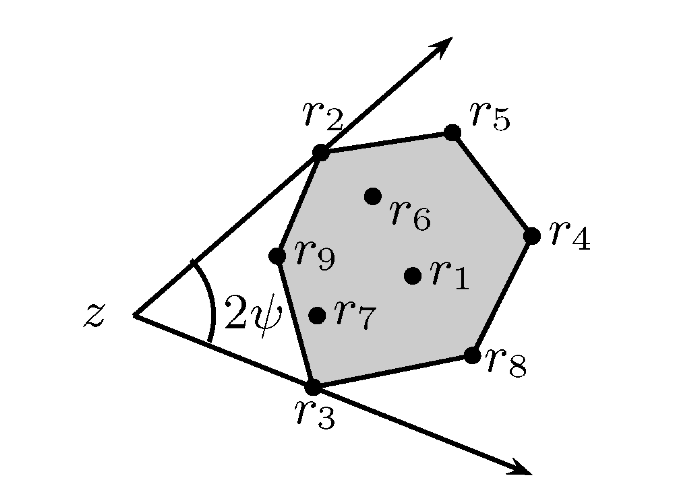
\includegraphics[width=0.5\textwidth]{fig_pb14.png}
	\\ Figura 5
\end{center}
Figura 5  Unghiul de vizualizare \(2\psi\) al acoperirii convexe a mulțimii rădăcinilor \(r_{1} , r_{2} , \cdots, r_{n}\)  lui \(P\left ( z \right )\), determină parametrul \(\psi\) pe care îl găsim în rafinarea cantitativă a lui Wilf a Teoremei Gauss-Lucas.
\end{problem}
\begin{proof}
Scriem \(r_{1} , r_{2} ,\cdots,r_{n}\) rădăcinile lui \(P\) repetate în funcție de multiplicitatea lor și pentru un \(z\) care se află în afara acoperirii convexe \(H\) scriem \(z - r_{j}\) în forma polară \(z - r_{j} = \rho _{j}e^{i\theta j}\). Atunci avem
\begin{displaymath}
  \frac{1}{z - r_{j}} = \rho _{j}^{-1}e^{-\theta ji} , 1 \leq  j \leq  n,
\end{displaymath}
și diferența între argumentele \(\theta _{j}, 1 \leq j\leq n\) este mai mică sau egală cu \(2\psi\). Astfel, din Inegalitatea  MA-MG forma complexă,avem
\begin{displaymath}
  \left ( \cos\psi  \right )\left | \frac{1}{z - r_{1}} \frac{1}{z - r_{2}}\cdots \frac{1}{z - r_{n}} \right|^{\frac{1}{n}} \leq  \frac{1}{n} \left | \sum_{j = 1}^{n}\frac{1}{z - r_{j}} \right |
\end{displaymath}
care în termeni de \(P\) si \({P}'\), se scrie că
\begin{displaymath}
   \left | \frac{a_{n}}{P\left ( z \right )} \right |^{\frac{1}{n}}\leq \frac{1}{n\cos\psi }\left | \frac{{P}'\left ( z \right )}{P\left ( z \right )} \right |,  \text{pentru orice }z \notin H,
\end{displaymath}
 ceea ce doream să demonstrăm.
\end{proof}

\begin{problem}
Dacă toate rădăcinile polinomului \(P\left ( z \right ) = a_{n}z^{n} +\cdots +a_{1}z + a_{0}\) sunt conținute în discul unitate \(U= \left \{ z: \left | z \right |\leq 1 \right \}\), atunci
\begin{displaymath}
    n\left | a_{n} \right |^{\frac{1}{n}}\left | P\left ( z \right ) \right |^{\frac{\left ( n-1 \right )}{n}}\sqrt{1 - \left | z \right |^{-2}}\leq \left | {P}'\left ( z \right ) \right |, \text{pentru orice } z\notin U. \label{eq:2.17} \tag{2.17}
\end{displaymath}
\end{problem}
\begin{proof}
Dacă \(2\psi\) este unghiul de vizualizare determinat de \(U\) când este privit din \(z \notin U\), atunci avem \(1 = \left | z \right |\sin\psi\), deci Teorema lui Pitagora ne spune că \(\cos\psi = \left ( 1 - \left | z \right |^{-2} \right )^{\frac{1}{2}}\). Inegalitatea  \ref{eq:2.17} rezultă apoi direct din inegalitatea lui Wilf, \ref{eq:2.16}.
\end{proof}
\begin{problem}
Arătați că dacă \(0 < r < 1\) și dacă numerele complexe \(z_{1}, z_{2},...,z_{n}\) sunt în discul \(D = \left \{ z: \left | z \right | \leq r\right \}\), atunci există \(z_{0} \in D\) astfel încât
\begin{displaymath}
    \prod_{j = 1}^{n}\left ( 1 + z_{j} \right ) = \left ( 1 + z_{0} \right )^{n}.\label{eq:2.18} \tag{2.18}
\end{displaymath}
\end{problem}
\begin{proof}
Discul \(D_{0} = \left \{ z : \left | 1 - z \right |\leq 1 \right \}\) scris în coordonate polare este
\begin{displaymath}
    \left \{ re^{i\theta }: 0 \leq r\leq 2\cos\theta , -\frac{\pi }{2}< \theta  < \frac{\pi }{2} \right \},
\end{displaymath}
deci pentru fiecare \(j\) putem scrie \(1 + z_{j}\) ca \(r_{j}e^{i\theta _{j}}\) unde \[-\frac{\pi }{2}< \theta  < \frac{\pi }{2},~r_{j}\leq 2\cos\theta _{j}.\]
 Rezultă imediat că \[z_{0} = -1 + \left ( r_{1} r_{2}\cdots r_{n}\right )^{\frac{1}{n}}exp\left ( i\frac{\left ( \theta _{1} + \theta _{2} +....+ \theta _{n} \right )}{n} \right )\] este soluția ecuației lui Nievergelt \ref{eq:2.18} și pentru a demonstra că \(z_{0}\in D \) este suficient să arătăm că \(1 + z_{0}\in D_{0}\), echivalent, trebuie să arătăm că
\begin{displaymath}
    \left ( r_{1} r_{2} \cdots r_{n}\right )^{\frac{1}{n}}\leq 2\cos\left ( \frac{\theta _{1} + \theta _{2}+\cdots+\theta _{n}}{n} \right ) \label{eq:2.19} \tag{2.19}.
\end{displaymath}
Cum \(\left ( r_{1} r_{2} \cdots r_{n}\right )^{\frac{1}{n}}\) este marginită de \(\left ( \left (2\cos\theta _{1}  \right )\left ( 2\cos\theta _{2} \right )\cdots \left (2\cos\theta _{n}  \right ) \right )^{\frac{1}{n}}\), este deci suficient să arătăm că
\begin{displaymath}
    \left ( \left (\cos\theta _{1}  \right )\left ( \cos\theta _{2} \right )\cdots \left (\cos\theta _{n}  \right ) \right )^{\frac{1}{n}}\leq \cos\left ( \frac{\theta _{1} + \theta _{2}+\cdots+\theta _{n}}{n} \right )
\end{displaymath}
și aceasta rezultă din concavitatea lui \(f\left ( x \right ) = \log \left ( \cos x \right ) pe -\frac{\pi }{2}< \theta < \pi\) împreună cu inegalitatea lui Jensen.
\end{proof}

\begin{problem} (Inegalitatea sumei ciclice a lui Shapiro)

Arătați că pentru orice numere pozitive
 \(a_{1} , a_{2} , a_{3}\)  si \(  a_{4}\), avem inegalitatea
 \begin{displaymath}
     2\leq \frac{a_{1}}{a_{2} + a_{3}} + \frac{a_{2}}{a_{3} + a_{4}} + \frac{a_{3}}{a_{4} + a_{1}} + \frac{a_{4}}{a_{1} + a_{2}} \label{eq:2.20} \tag{2.20}
 \end{displaymath}
 \end{problem}
 \begin{remark}
De altfel,  Bushell (1994) ne oferă o mulțime de informații despre inegalități de forma
\begin{displaymath}
    \frac{n}{2} \leq \frac{x_{1}}{x_{2} + x_{3}} + \frac{x_{2}}{x_{3} + x_{4}} + \cdots+ \frac{x_{n - 1}}{x_{n} + x_{1}} + \frac{x_{n}}{x_{1} + x_{2}}.
\end{displaymath}
Se știe că această inegalitate nu este adevarată pentru  \(n\geq 25\), totuși mulțimea precisă a valorilor lui n pentru care este adevarată, nu a fost încă determinată.
\end{remark}
\begin{proof}
O soluție frumoasă folosind inegalitatea lui Jensen pentru \(f\left ( x \right ) = \frac{1}{x}\) a fost dată de Robert Israel în grupul de știri sci.math în 1999.

Dacă notăm \(S = a_{1} + a_{2} + a_{3} + a_{4}\) si \(C\) reprezintă suma din partea dreaptă a inegalității \ref{eq:2.18}, atunci Inegalitatea lui Jensen cu \(p_{j} = \frac{a_{j}}{S}\) și
\[x_{1} = a_{2} + a_{3}, x_{2} = a_{3} + a_{4}, x_{3} = a_{4} + a_{1},~x_{4} = a_{1} + a_{2}\] conduce la
\[\frac{C}{S} \geq \left \{ \frac{D}{S} \right \}^{-1}\]
 sau \(C \geq \frac{S^{2}}{D}\), unde am notat
\begin{displaymath}
    D = a_{1}\left ( a_{2} + a_{3} \right ) + a_{2}\left ( a_{3} + a_{4} \right ) + a_{3}\left ( a_{4} + a_{1} \right ) + a_{4}\left ( a_{1} + a_{2} \right ).
\end{displaymath}
Acum, este simplu să verificăm că
\begin{displaymath}
    S^{2} - 2D = \left ( a_{1} - a_{3} \right )^{2} + \left ( a_{2} - a_{4} \right )^{2}> 0.
\end{displaymath}
Acest lucru este suficient pentru a completa soluția.
\end{proof}

\begin{problem} (Lema celor trei coarde)
Arătați că dacă \(f : \left [ a,b \right ]  \to \mathbb{R}\) este convexă și \(a <  x < b\), atunci avem
\begin{displaymath}
    \frac{f\left ( x \right ) - f\left ( a \right )}{x - a} \leq \frac{f\left ( b \right ) - f\left ( a \right )}{b - a} \leq  \frac{f\left ( b \right ) - f\left ( x \right )}{b - x}.   \label{eq:2.21}\tag{2.21}
\end{displaymath}
\end{problem}
\begin{proof}
Din convexitate avem
\begin{displaymath}
    x = \frac{b - x}{b - a}a + \frac{x - a}{b - a }b \Rightarrow f\left ( x \right ) \leq \frac{b - x}{b - a}f\left ( a \right ) + \frac{x - a}{b - a }f\left ( b \right )
\end{displaymath}
 deci, după scăderea lui \(f\left ( a \right )\), va rezulta
 \begin{displaymath}
     f\left ( x \right ) - f\left ( a \right )\leq \frac{x - a}{b - a }\left \{ f\left ( b \right ) - f\left ( a \right ) \right \}. \label{eq:2.22} \tag{2.22}
 \end{displaymath}
Aceasta ne dă a doua inegalitate din \ref{eq:2.21} iar prima inegalitate se demonstrează în același mod.
\end{proof}








\bibliographystyle{unsrt}
\setlength{\baselineskip}{\normalbaselineskip}
\setlength{\parskip}{0pt}
\bibliography{refs}
\end{document}














\begin{problem} (Lema celor trei coarde)
Arătați că dacă \(f : \left [ a,b \right ]  \to \mathbb{R}\) este convexă și \(a <  x < b\), atunci avem
\begin{displaymath}
    \frac{f\left ( x \right ) - f\left ( a \right )}{x - a} \leq \frac{f\left ( b \right ) - f\left ( a \right )}{b - a} \leq  \frac{f\left ( b \right ) - f\left ( x \right )}{b - x}.   \label{eq:2.21}\tag{2.21}
\end{displaymath}
\end{problem}
\begin{remark}
Așa cum ne sugerează următoarele două exerciții, această limită este cheia pentru câteva dintre cele mai de bază proprietăți de regularitate ale funcțiilor convexe.
\end{remark}
Prin interpolare și convexitate avem
\begin{displaymath}
    x = \frac{b - x}{b - a}a + \frac{x - a}{b - a }b \Rightarrow f\left ( x \right ) \leq \frac{b - x}{b - a}f\left ( a \right ) + \frac{x - a}{b - a }f\left ( b \right )
\end{displaymath}
 deci, după scaderea lui \(f\left ( a \right )\), avem
 \begin{displaymath}
     f\left ( x \right ) - f\left ( a \right )\leq \frac{x - a}{b - a }\left \{ f\left ( b \right ) - f\left ( a \right ) \right \}. \label{eq:2.22} \tag{2.22}
 \end{displaymath}
Aceasta ne da a doua inegalitate a \ref{eq:2.21} iar cea de a doua este demonstrată în același mod.


Problema 21

Aproape diferențiabilitatea funcțiilor convexe

Folosind Lema celor trei coarde pentru a arăta că pentru funcția convexă \(f : \left [ a,b \right ]  \to \mathbb{R}\) si \(a< x< b\) există limite finite
\begin{displaymath}
    {f}'_{+} + \left ( x \right ) = \lim_{h  \to 0}\frac{f\left ( x + h \right ) - f\left ( x \right )}{h}
\end{displaymath}
și
\begin{displaymath}
    {f}'_{-} + \left ( x \right ) = \lim_{h  \to 0}\frac{f\left ( x - h \right ) - f\left ( x \right )}{h}.
\end{displaymath}
Fie
\begin{displaymath}
    g\left ( h \right ) = \frac{\left \{ f\left ( x + h \right ) - f\left ( x \right ) \right \}}{h}
\end{displaymath}
 și verificăm de la Lema celor trei coarde că pentru \(0 < h_{1} < h_{2}\) avem \(g\left ( h_{1} \right )\leq g\left ( h_{2} \right )\). Mai departe luăm \(y\) cu \(a <  y < x \) și folosim Lema celor trei coarde pentru a verifica că
 \begin{displaymath}
    -\infty < \frac{\left \{ f\left ( x \right ) - f\left ( y \right ) \right \}}{x - y}\geq g\left ( h \right )
 \end{displaymath}
 pentru orice \(h> 0\). Monotonitatea și mărginirea \(g\left ( h \right )\) garantează faptul că \(g\left ( h \right )\) are limită finită în \(h \to 0\). Acest lucru ne oferă prima jumatate a problemei, iar cea de a doua aproape identic.

Problema 22

Limitele de raport și minoranții liniari

Pentru funcțiile convexe \(f : \left [ a,b \right ]  \to \mathbb{R}\) si \(a< x<y< b\), aratați că există
\begin{displaymath}
   {f}'_{-}\left ( x \right ) \leq  {f}'_{+}\left ( x \right ) \leq  \frac{f\left ( y \right ) - f\left ( x \right )}{y - x} \leq  {f}'_{-}\left ( y \right ) \leq  {f}'_{+}\left ( y \right ) \label{eq:2.23} \tag{2.23}
\end{displaymath}

În particular, observăm că pentru orice
\begin{displaymath}
   \theta \in \left [ {f}'_{-}\left ( x \right ), {f}'_{+}\left ( x \right ) \right ],
\end{displaymath}
 avem limita
 \begin{displaymath}
(f\left ( y \right ) \geq  f\left ( x \right ) + \left ( y - x \right )\theta \text{pentru orice  }y\in \left [ a,b \right ]. \label{eq:2.24} \tag{2.24}
 \end{displaymath}

Limita inferioară liniară \ref{eq:2.22} este mai eficientă decât sugerează simplitatea sa și are câteva consecințe notabile.
Aceasta este doar o lucrare mai la îndemână a Teoremei celor trei coarde care ne dă pentru \(0< s\) și \(0< t\) cu \(y - s \in I\) si \(y + t  \in I\) faptul că
\begin{displaymath}
   \frac{f\left ( y \right ) - f\left ( y - s \right )}{s}\leq \frac{f\left ( y + t \right ) - f\left ( y \right )}{t}.
\end{displaymath}
 De la exercițiul 21 avem acele limite finite ca \(s,t \to 0\), și aceste limite sunt \({f}'_{-}\left ( y \right )\) și respectiv \({f}'_{+}\left ( y \right )\). Acest lucru ne oferă faptul că \({f}'_{-}\left ( y \right )\leq {f}'_{+}\left ( y \right )\) și celelalte limite nu sunt mai grele. Identic, limita \({f}'_{-}\left ( y \right )\leq {f}'_{+}\left ( y \right )\) poate fi privită ca o versiune infimă a Lemei celor trei coarde.
Pentru \(a < x \leq s\leq t\leq y<  b\) și \( M = max\left \{ \left | {f}'_{+} \left ( x \right )\right |,\left | {f}'_{-} \left ( y \right )\right |  \right \}\) limita \ref{eq:2.21} ne oferă \(\left | f\left ( t \right ) - f\left ( s \right ) \right |\leq M\left | t - s \right |\), care este mai mult decât aveam nevoie pentru a spune ca f este conutinuă.


